\documentclass[times,specification,annotation]{itmo-student-thesis}

%% Опции пакета:
%% - specification - если есть, генерируется задание, иначе не генерируется
%% - annotation - если есть, генерируется аннотация, иначе не генерируется
%% - times - делает все шрифтом Times New Roman, собирается с помощью xelatex
%% - languages={...} - устанавливает перечень используемых языков. По умолчанию это {english,russian}.
%%                     Последний из языков определяет текст основного документа.

%% Делает запятую в формулах более интеллектуальной, например:
%% $1,5x$ будет читаться как полтора икса, а не один запятая пять иксов.
%% Однако если написать $1, 5x$, то все будет как прежде.
\usepackage{icomma}

%% Один из пакетов, позволяющий делать таблицы на всю ширину текста.
\usepackage{tabularx}

%% Пакет для создания диагональных разделяющих линий в ячейках таблиц.
\usepackage{diagbox}

%% Пакет для работы с библиографией
\usepackage{filecontents}
\begin{filecontents}{bachelor-thesis.bib}
@inproceedings{ neuront,
    author={Игорь Сергеевич Подцепко and Евгений Александрович Беляев},
    title={Транскодирование JPEG-изображений при помощи нейросетевого предсказания коэффициентов ДКП},
    journal={Сборник конференции NeuroNT'2024},
    year={2024},
    note={Принята к публикации},
    langid={russian}
}

@article{ jpeg-standard,
    author={G. K. Wallace},
    title={The jpeg still picture compression standard},
    journal={Commun. ACM},
    volume={34},
    number={4},
    month={4},
    year={1991},
    pages={30–44},
    language={english},
    langid={english}
}

@article{ jpeg-overview,
    author={G. K. Wallace},
    title={Overview of the JPEG (ISO/CCITT) still image compression standard},
    journal={Proc. SPIE},
    volume={1244},
    month={6},
    year={1990},
    pages={220–233},
    language={english},
    langid={english}
}

@article{ jpeg2000-overview,
    author={C. Christopoulos and A. Skodras and T. Ebrahimi},
    title={The jpeg2000 still image coding system: an overview},
    journal={IEEE Transactions on Consumer Electronics},
    volume={46},
    number={4},
    year={2000},
    pages={1103–1127},
    language={english},
    langid={english}
}

@article{ hevc-overview,
    author={G. J. Sullivan and J.-R. Ohm and W.-J. Han and T. Wiegand},
    title={Overview of the high efficiency video coding (HEVC) standard},
    journal={IEEE Trans. Circuits Syst. Video Technol.},
    volume={22},
    number={12},
    month={12},
    year={2012},
    pages={1649–1668},
    language={english},
    langid={english}
}

@article{ jpeg-ls-overview,
    author={M. J. Weinberger and G. Seroussi and G. Sapiro},
    title={The LOCO-I lossless image compression algorithm: Principles and standardization into JPEG-LS},
    journal={IEEE Trans. Image Process.},
    volume={9},
    number={8},
    month={8},
    year={2000},
    pages={1309–1324},
    language={english},
    langid={english}
}

@online{ bpg-website,
    author={F. Bellard},
    title={BPG Image Format Website},
    url={http://bellard.org/bpg/},
    year={2024},
    langid={english}
}

@article{ calic-overview,
    month={5},
    year={1996},
    booktitle={Proc. IEEE Int. Conf. Acoust., Speech, Signal Process. (ICASSP)},
    author={X. Wu and N. Memon},
    title={CALIC—A context based adaptive lossless image codec},
    pages={1890–1893},
    language={english},
    langid={english}
}

@online{ flif-website,
    author={J. Sneyers},
    title={FLIF Image Format Website},
    url={http://flif.info/},
    year={2024},
    langid={english}
}

@online{ tinypng-project,
    author={A. Kyleduo},
    title={Tinypng Project},
    url={https://tinypng.com/developers},
    year={2024},
    langid={english}
}

@online{ mozjpeg-github-page,
    author={Mozilla},
    title={Mozilla Mozjpeg},
    url={https://github.com/mozilla/mozjpeg},
    year={2024},
    langid={english}
}

@online{ pytorch,
    author={The Linux Foundation},
    title={PyTorch},
    url={https://pytorch.org/},
    year={2024},
    langid={english}
}

@online{ mozilla-comparison-of-compression-formats,
    author={Mozilla},
    title={Lossy Compressed Image Formats Study},
    url={https://web.archive.org/web/20160311235158/http://people.mozilla.org/~josh/lossy_compressed_image_study_july_2014},
    month={7},
    year={2024},
    langid={english}
}

@online{ webp-overview,
    author={Google},
    title={An image format for the Web},
    url={https://developers.google.com/speed/webp},
    year={2024},
    langid={english}
}


@misc{ guetzli-overview,
    author={Jyrki Alakuijala and Robert Obryk and Ostap Stoliarchuk and Zoltan Szabadka and Lode Vandevenne and Jan Wassenberg},
    title={Guetzli: Perceptually Guided JPEG Encoder},
    year={2017},
    eprint={1703.04421},
    archivePrefix={arXiv},
    primaryClass={cs.CV}
}

@article{ lljpeg-overview,
    author={C. Sun and X. Fan and D. Zhao},
    title={Lossless Recompression of JPEG Images Using Transform Domain Intra Prediction},
    journal={IEEE Transactions on Image Processing},
    volume={32},
    year={2023},
    pages={88-99},
    language={english},
    langid={english}
}

@online{ lljpeg-testing,
    author={vilab-sct},
    title={LLJPEG},
    url={https://github.com/vilab-sct/LLJPEG},
    year={2022},
    langid={english}
}

@online{ args-lib,
    author={Taywee},
    title={args},
    url={https://github.com/Taywee/args},
    year={2024},
    langid={english}
}

@online{ jpegtran-description,
    author={H. Kulissen},
    title={Jpegtran Description},
    url={http://jpegclub.org/articles/Verlustfreie_JPEG_Drehung.pdf},
    year={2024},
    langid={english}
}

@online{ jpegtran-project,
    author={H. Kulissen},
    title={Jpegtran Project},
    url={https://www.npmjs.com/package/jpegtran},
    year={2024},
    langid={english}
}

@online{ ai-video-enhancement,
    author={Evgeny Belyaev},
    title={AIVideoEnhancement},
    url={https://gitlab.actcognitive.org/aivideocoding/aivideoenhancement},
    year={2024},
    langid={english}
}

@article{ image-net,
    author={J. Deng and W. Dong and R. Socher and L.-J. Li and K. Li and L. Fei-Fei},
    title={ImageNet: A Large-Scale Hierarchical Image Database},
    journal={CVPR09},
    year={2009},
    language={english},
    langid={english}
}

@article{ qe-cnn-overview,
   title={Enhancing Quality for HEVC Compressed Videos},
   volume={29},
   ISSN={1558-2205},
   url={http://dx.doi.org/10.1109/TCSVT.2018.2867568},
   DOI={10.1109/tcsvt.2018.2867568},
   number={7},
   journal={IEEE Transactions on Circuits and Systems for Video Technology},
   publisher={Institute of Electrical and Electronics Engineers (IEEE)},
   author={Yang, Ren and Xu, Mai and Liu, Tie and Wang, Zulin and Guan, Zhenyu},
   year={2019},
   month=jul,
   pages={2039–2054}
}

@misc{ ar-cnn-overview,
    title={Compression Artifacts Reduction by a Deep Convolutional Network},
    author={Chao Dong and Yubin Deng and Chen Change Loy and Xiaoou Tang},
    year={2015},
    eprint={1504.06993},
    archivePrefix={arXiv},
    primaryClass={cs.CV}
}

@book{ information-theory,
    author      = {Б. Д. Кудряшов},
    title       = {Теория информации},
    address     = {Санкт-Петербург},
    publisher   = {СПбГУ ИТМО},
    numpages    = {188},
    pagetotal   = {188},
    year        = {2010},
    langid      = {russian}
}

@misc{jeon2023contextbased,
      title={Context-Based Trit-Plane Coding for Progressive Image Compression},
      author={Seungmin Jeon and Kwang Pyo Choi and Youngo Park and Chang-Su Kim},
      year={2023},
      eprint={2303.05715},
      archivePrefix={arXiv},
      primaryClass={eess.IV}
}

@misc{feng2023nvtc,
      title={NVTC: Nonlinear Vector Transform Coding},
      author={Runsen Feng and Zongyu Guo and Weiping Li and Zhibo Chen},
      year={2023},
      eprint={2305.16025},
      archivePrefix={arXiv},
      primaryClass={cs.CV}
}

@misc{huang2023accurate,
      title={Towards Accurate Image Coding: Improved Autoregressive Image Generation with Dynamic Vector Quantization},
      author={Mengqi Huang and Zhendong Mao and Zhuowei Chen and Yongdong Zhang},
      year={2023},
      eprint={2305.11718},
      archivePrefix={arXiv},
      primaryClass={cs.CV}
}

\end{filecontents}

%% Указываем файл с библиографией.
\addbibresource{bachelor-thesis.bib}

\begin{document}

\studygroup{M34381}
\title{Транскодирование JPEG-изображений при помощи предсказания коэффициентов ДКП на основе нейронной сети}
\author{Подцепко Игорь Сергеевич}{Подцепко И.С.}
\supervisor{Беляев Евгений Александрович}{Беляев Е.А.}{PhD}{науки, Университет ИТМО, факультет информационных технологий и программирования, доцент (квалификационная категория "ординарный доцент")}
\publishyear{2024}
%% Дата выдачи задания.
\startdate{31}{января}{2024}
%% Срок сдачи студентом работы.
\finishdate{30}{апреля}{2024}
%% Дата защиты.
%% \defencedate{15}{июня}{2024}

%% Секретарь ГЭК.
\secretary{Штумпф С.А.}

%% Задание

%%% Техническое задание и исходные данные к работе
\technicalspec{
    Разработать и обучить нейронную сеть, которая предсказывает часть коэффициентов дискретного косинусного преобразования (ДКП) из входного JPEG-изображения, и использовать полученные коэффициенты для энтропийного кодирования исходных коэффициентов.
}

%%% Содержание выпускной квалификационной работы (перечень подлежащих разработке вопросов)
\plannedcontents{
    Изучить возможность и потенциал нейронных сетей для реализации этапа внутреннего предсказания коэффициентов ДКП при транскодировании JPEG-изображений.\par

    Задачи работы:
    \begin{enumerate}
        \item Реализовать декодирование JPEG-изображений с удалением (обнулением) части коэффициентов ДКП для подготовки набора данных для обучения нейронной сети;
        \item Разработать и обучить нейронную сеть, которая предсказывает (вычисляет) часть коэффициентов ДКП на основании остальных коэффициентов;
        \item Реализовать кодирование с предсказанием для сжатия выбранной части коэффициентов ДКП;
        \item Оценить степень сжатия, которую удается достичь благодаря нейросетевому внутреннему предсказанию.
    \end{enumerate}
}

%%% Исходные материалы и пособия
\plannedsources{}

%%% Цель исследования
\researchaim{Изучить возможность и потенциал нейронных сетей для реализации этапа внутреннего предсказания коэффициентов ДКП при транскодировании JPEG-изображений.}

%%% Задачи, решаемые в ВКР
\researchtargets{
    \begin{enumerate}
        \item Реализовать декодирование JPEG-изображений с удалением (обнулением) части коэффициентов ДКП для подготовки набора данных для обучения нейронной сети;
        \item Разработать и обучить нейронную сеть, которая предсказывает (вычисляет) часть коэффициентов ДКП на основании остальных коэффициентов;
        \item Реализовать кодирование с предсказанием для сжатия выбранной части коэффициентов ДКП;
        \item Оценить степень сжатия, которую удается достичь благодаря нейросетевому внутреннему предсказанию.
    \end{enumerate}
}

%%% Использование современных пакетов компьютерных программ и технологий
\addadvancedsoftware{\texttt{PyTorch} --- фреймворк машинного обучения для языка Python.}{Разработка и обучение нейронной сети для улучшения изображений.}

%%% Краткая характеристика полученных результатов
\researchsummary{
    Разработан метод внутреннего предсказания коэффициентов ДКП для транскодирования JPEG-изображений, основанный на применении нейронной сети и позволяющий сократить размер JPEG-файлов из подмножества набора данных ImageNet в среднем на 3,33\% при медиане 3,38\%. Наилучшее достигнутое сжатие составило 6,28\%. Метод успешно комбинируется с утилитой Jpegtran, позволяющей заменять код Хаффмана на арифметическое кодирование, и общая степень сжатия в среднем составляет 13,16\%.
}

%%% Гранты, полученные при выполнении работы
\researchfunding{}

%%% Наличие публикаций и выступлений на конференциях по теме выпускной работы
\researchpublications{}

%% Эта команда генерирует титульный лист и аннотацию.
\maketitle{Бакалавр}

%% Оглавление
\tableofcontents

%% Макрос для введения. Совместим со старым стилевиком.
\startprefacepage

JPEG --- это стандарт сжатия изображений, который был разработан в 1992 году Joint Photographic Experts Group. До настоящего времени он остается наиболее распространенным форматом сжатия изображений из-за своей низкой вычислительной сложности, однако качество сжатия JPEG значительно уступает более современным алгоритмам, таким как WebP, HEIF, AVIF и т. д.\par

В современном мире цифровых устройств фотографии, сохраненные в формате JPEG, стали неотъемлемой частью социальной жизни. С каждым днем все больше людей используют социальные сети, такие как ВКонтакте и Telegram, для обмена сообщениями и изображениями. Эти веб-сайты хранят огромное число JPEG-изображений на своих серверах. Более того, массовое использование JPEG-изображений приводит к увеличению спроса на локальные и облачные хранилища. Следовательно, исследование способов снижения затрат на хранение JPEG-изображений в облачном хранилище или на персональных компьютерах становится все более важной и актуальной задачей. При этом чаще всего речь идет именно о более эффективном хранении без потерь, так как если пользователь загружает в облачное хранилище изображение — он ожидает получить его в будущем в неизменном виде. \par

Для решения проблемы хранения больших объемов изображений JPEG транскодер может использоваться, как показано на рисунке~\ref{cloud-storage-system}. При загрузке в облачное хранилище JPEG файл дополнительно сжимается без потерь транскодером, а при запросе от пользователя трансдекодируется в исходное представление.\par

\begin{figure}[!h]
    \centering
    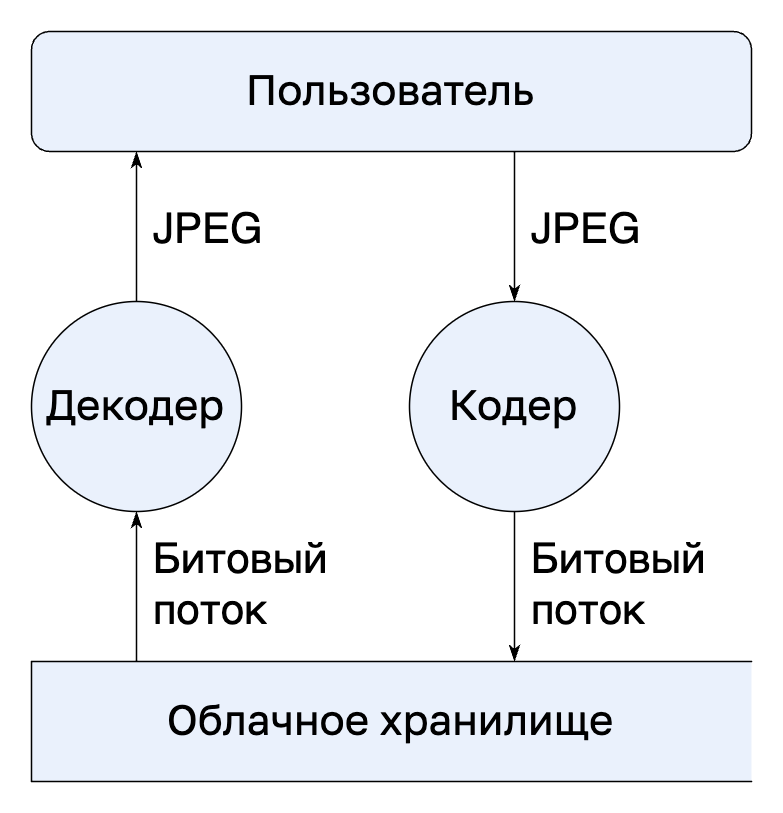
\includegraphics[width=9cm]{./images/cloud-storage-system.png}
    \caption{Архитектура внедрения транскодера JPEG}
    \label{cloud-storage-system}
\end{figure}

Настоящая работа рассматривает алгоритм внутреннего предсказания ДКП-коэффициентов с помощью нейронной сети. В процессе работы предлагаемого алгоритма JPEG изображение декодируется до коэффициентов ДКП, после чего часть из них обнуляется. Такое преобразование вносит в изображения определенные искажения, которые могут исправляться специально обученной нейронной сетью. В области коэффициентов ДКП это соответствует появлению на местах обнуленных коэффициентов значений близких к исходным. Далее на места обнуленных коэффициентов записываются ошибки их предсказания, и изображение кодируется энтропийным кодером из алгоритма JPEG. На выходе транскодера получается корректный файл JPEG, но меньшего объема. Данный подход позволяет лучше устранять избыточность, возникающую между блоками изображения, так как реализует предсказание не только DC, но и AC-коэффициентов. Метод является совместимым с другими существующими транскодерами JPEG и в среднем позволяет добиться сжатия на 3,33\%.\par

Цель работы: Изучить возможность и потенциал нейронных сетей для реализации этапа внутреннего предсказания коэффициентов ДКП при транскодировании JPEG-изображений.
\par

Задачи работы:
\begin{enumerate}
    \item Реализовать декодирование JPEG-изображений с удалением (обнулением) части коэффициентов ДКП для подготовки набора данных для обучения нейронной сети;
    \item Разработать и обучить нейронную сеть, которая предсказывает (вычисляет) часть коэффициентов ДКП на основании остальных коэффициентов;
    \item Реализовать кодирование с предсказанием для сжатия выбранной части коэффициентов ДКП;
    \item Оценить степень сжатия, которую удается достичь благодаря нейросетевому внутреннему предсказанию.
\end{enumerate}

%% TODO: Актуализировать описание структуры работы после завершения работы над документом.
Настоящая работа имеет следующую структуру. В первой главе рассматриваются существующие алгоритмы сжатия изображений: JPEG, JPEG2000, HEVC, JPEG-LS и другие. Также в этой главе приводится краткая сводка относительно существующих на сегодняшний день подходов к транскодированию JPEG-изображений с потерями и без потерь, формулируются основные подходы к решению данной задачи. Вторая глава содержит мотивацию, краткий обзор и более подробное описание предлагаемого алгоритма транскодирования. В третьей главе приводится детальная информация о том, как было реализовано декодирование JPEG-изображений с обнулением коэффициентов, описываются детали реализации и обучения нейронной сети, а также содержатся результаты экспериментов по оценке степени сжатия предлагаемым алгоритмом и сравнение его с другими подходами.

%% Начало содержательной части.
\chapter{Постановка задачи о транскодировании JPEG-изображений и обзор существующих решений}\label{chapter:theory}

В данной главе приводится постановка задачи транскодирования JPEG-изображений и рассматривается непосредственно алгоритм JPEG. Описывается схема и принцип работы транскодера, основанного на применении методов машинного обучения.

\startrelatedwork

\section{Алгоритм JPEG}\label{sec:jpeg}

При сжатии алгоритмом JPEG~\cite{jpeg-overview} изображение проходит несколько этапов преобразования, показанных на рисунке~\ref{image:jpeg-overview}. В данном разделе рассматривается каждый из этапов кодирования.

\begin{figure}[!h]
    \centering
    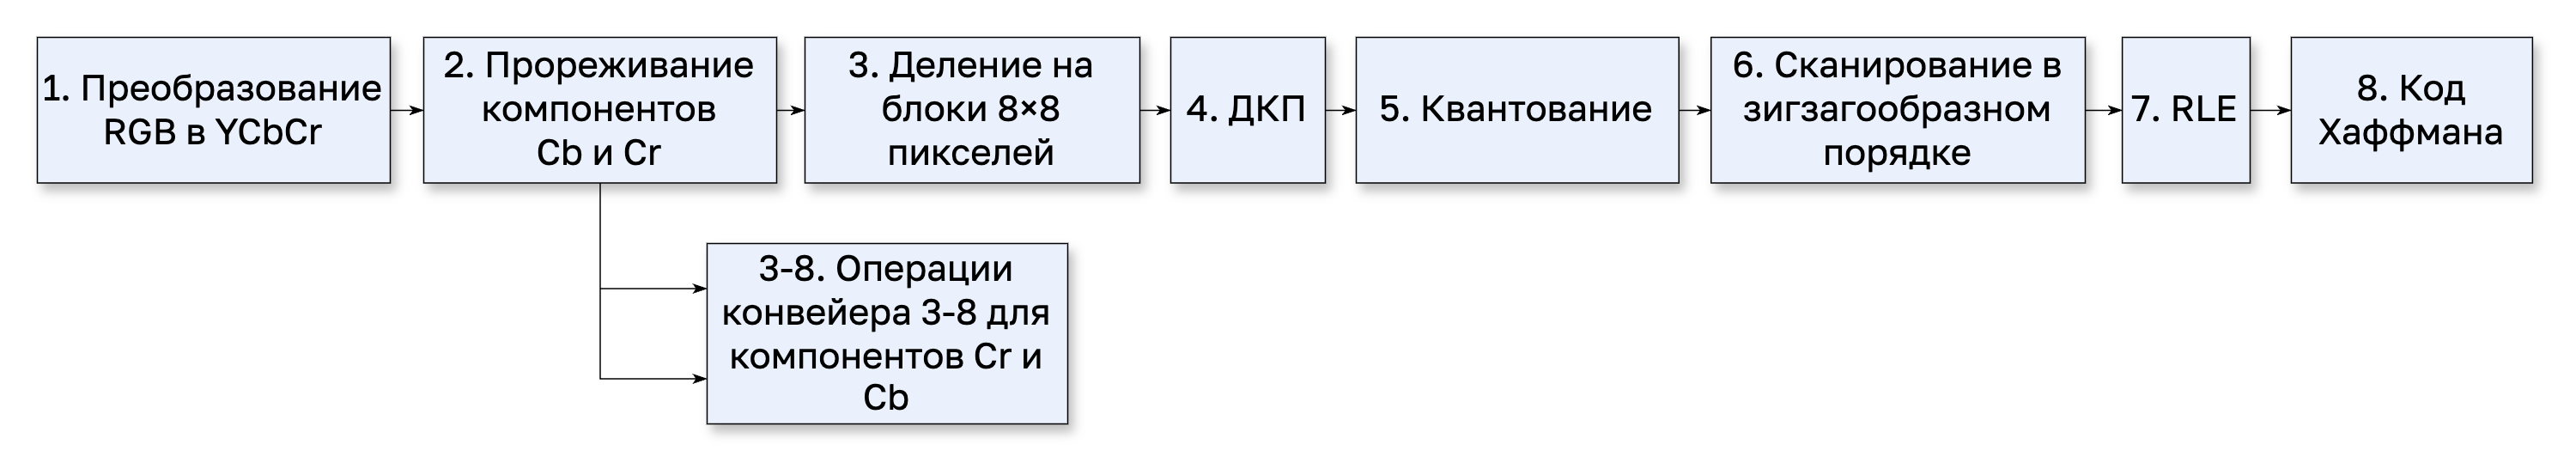
\includegraphics[width=\textwidth]{./images/jpeg-overview.png}
    \caption{Стадии алгоритма JPEG}
    \label{image:jpeg-overview}
\end{figure}

\subsection{Преобразование цветового пространства}\label{subsec:color-space-conversion}

На первом этапе работы JPEG изображение переводится из цветового пространства RGB в YCbCr:\par

\begin{equation*}
    \begin{cases}
        Y = 0.299 \cdot R + 0.587 \cdot G + 0.114 \cdot B - 128 \\
        Cb = -0.16874 \cdot R - 0.33126 \cdot G + 0.5 \cdot B   \\
        Cr = 0.5 \cdot R - 0.41869 \cdot G - 0.08131 \cdot B
    \end{cases}
\end{equation*}

Компонент Y (luminance) представляет собой яркостную характеристику пикселя и определяет его интенсивность. Он кодирует черно-белую информацию изображения. Компоненты Cb (chroma blue) и Cr (chroma red) вычисляются как разности между цветом пикселя и его яркостью, то есть являются цветовыми компонентами (или каналами). Визуализация данного представления показана на рисунке~\ref{image:yuv-example}.\par

\begin{figure}[!h]
    \centering
    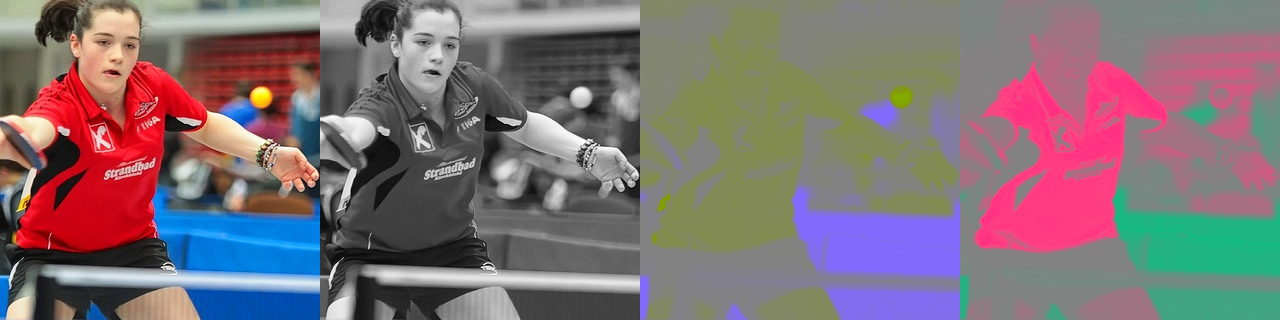
\includegraphics[width=\textwidth]{./images/yuv-example.png}
    \caption{Слева направо: исходное изображение, Y, Cb, Cr}
    \label{image:yuv-example}
\end{figure}

Преимущество YCbCr состоит в том, что в силу особенностей зрительной системы человека значимость яркости превышает значимость цвета. Другими словами, наш глаз лучше фиксирует изменения именно в яркостном компоненте. Это говорит о психовизуальной избыточности. По этой причине на втором шаге алгоритма JPEG выполняется прореживание (субдискретизация) цветовых компонентов.

\subsection{Цветовая субдискретизация}\label{subsec:chroma-subsampling}

Цветовая субдискретизация --- это уменьшение размерностей цветовых каналов, с целью снижения размера итогового цифрового потока. Фактически это означает, что частота выборки для цветовых компонентов оказывается меньше, чем для яркостного компонента.\par

Существуют различные форматы субдискретизации (рисунок~\ref{image:subsampling-examples}). Структура дискретизации изображения описывается соотношением между тремя частями $n:m_1:m_2$. Этими частями являются:
\begin{itemize}
    \item $n$ --- частота дискретизации канала Y (ширина макропикселя);
    \item $m_1$ --- число выборок каналов Cr, Cb в горизонтальном направлении в первой строке;
    \item $m_1$ --- число выборок каналов Cr, Cb в горизонтальном направлении во второй строке;
\end{itemize}

\begin{figure}[!h]
    \centering
    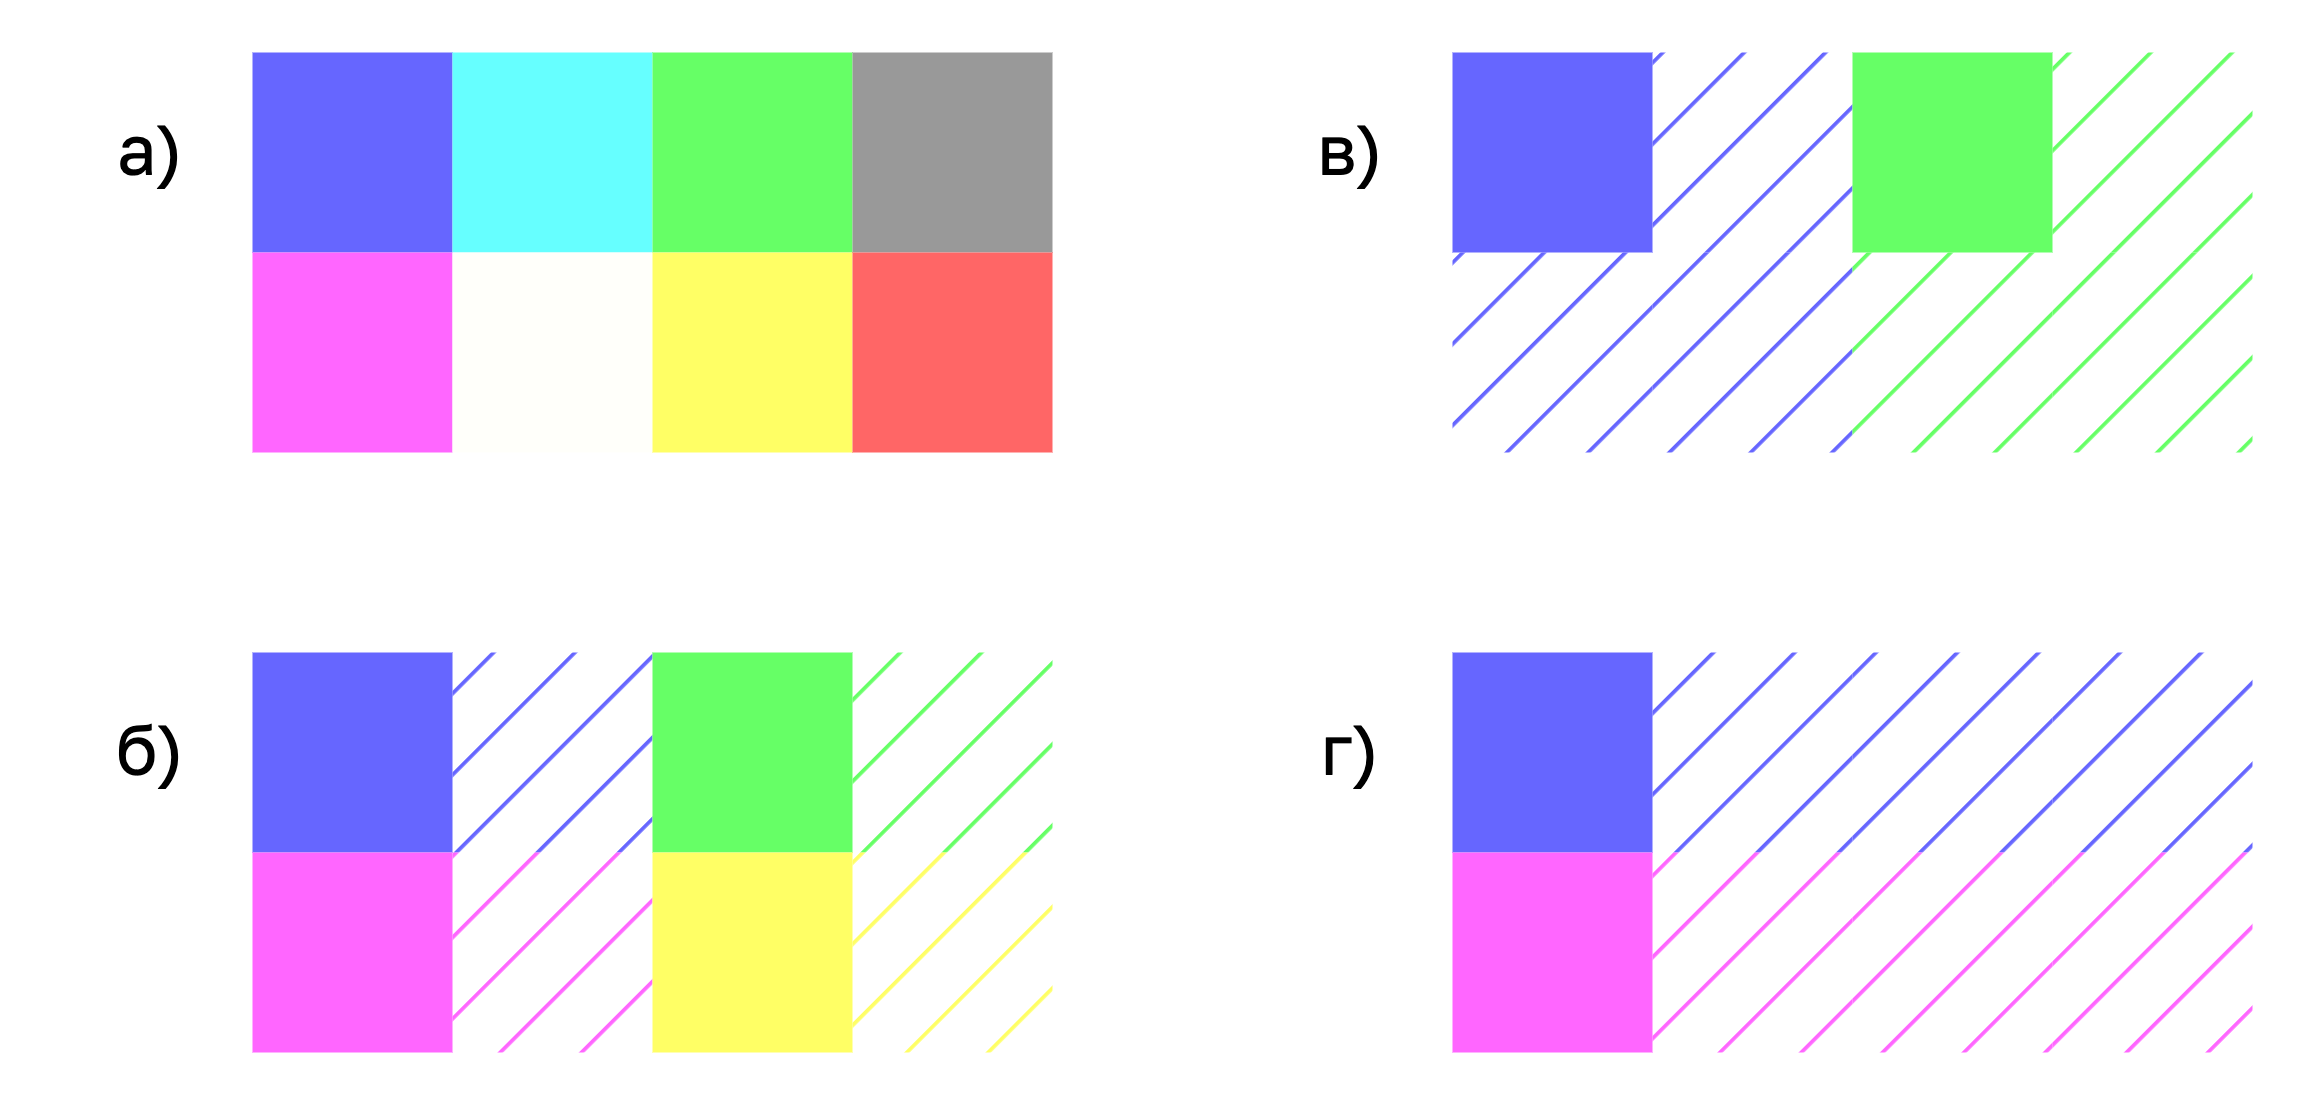
\includegraphics[width=10cm]{./images/subsampling-examples.png}
    \caption{Различные форматы субдискретизации:\\
        а) $4:4:4$; б) $4:2:2$; в) $4:2:0$; г) $4:1:1$}
    \label{image:subsampling-examples}
\end{figure}

\subsection{Деление на блоки и дискретное косинусное преобразование}\label{subsec:block-partition-and-dct}

После прореживания каждый из компонентов делится на блоки $8\times8$ пикселей, которые кодируются отдельно и независимо друг от друга. К ним применяется двумерное дискретное косинусное преобразование (ДКП) --- метод преобразования сигналов (изображений) из пространства времени (пикселей) в пространство частот, использующее косинусные функции для разложения сигнала на сумму синусоид с разными частотами. Вычисляется ДКП по следующей формуле:

$$g(x, y, u, v) = h(x, y, u, v) = a(u)a(v)\cos\left(\dfrac{(2x + 1)u\pi}{2N}\right)\cos\left(\dfrac{(2y + 1)v\pi}{2N}\right),$$
где
\begin{equation*}
    a(u) = \begin{cases}
        \dfrac{1}{\sqrt{N}}, & u = 0,    \\
        \dfrac{2}{\sqrt{N}}, & u \neq 0.
    \end{cases}
\end{equation*}

Коэффициенты, полученные после ДКП, разделяют на:
\begin{itemize}
    \item DC-коэффициент (или коэффициент постоянной составляющей), находящийся в верхнем левом углу блока --- компонент, отвечающий за среднее значение яркости или интенсивности цвета блока;
    \item AC-коэффициенты --- высокочастотные компоненты блока, причем чем больше сумма индексов коэффициента --- тем более высокочастотный компонент он описывает.
\end{itemize}

\subsection{Квантование}\label{subsec:quantization}

Следующим этапом работы алгоритма JPEG является квантование --- это поэлементное деление коэффициентов ДКП на матрицы квантования с округлением вниз. Как правило, для каждого компонента изображения используется собственная матрица квантования. Абсолютные значения элементов матриц зависят от параметра качества (quality factor, QF), передаваемого кодеру JPEG, однако обычно более высокочастотные коэффициенты ДКП квантуются сильнее. Более того, на практике многие из них обнуляются.\par

\subsection{Кодирование DC-коэффициентов}\label{subsec:dc-coding}

После квантования применяется кодирование с предсказанием: каждый DC-коэффициент (кроме первого) заменяется на разность между квантованным текущим и предыдущим DC-коэффициентами из того же канала. Преимущество такого подхода по сравнению с кодированием самих значений DC-коэффициентов состоит в том, что он позволяет устранять избыточность между соседними блоками, возникающую из-за того, что в реальных изображениях можно наблюдать самоподобие и средние значения яркости/цвета соседних блоков часто близки друг к другу.\par

\subsection{Энтропийное кодирование}\label{subsec:entropy-coding}

После этапа квантования и внутреннего предсказания DC-коэффициентов применяется кодирование длин серий (run-level encoding, RLE), в процессе которого коэффициенты сканируются в зигзагообразном порядке, показанном на рисунке~\ref{image:zigzag-order}, и последовательности из $run$ нулей и ненулевого коэффициента со значением $x$ заменяются на пару $(run,\ level)$, где $level$ --- длина двоичного представления $x$ в прямом коде.\par

\begin{figure}[!h]
    \centering
    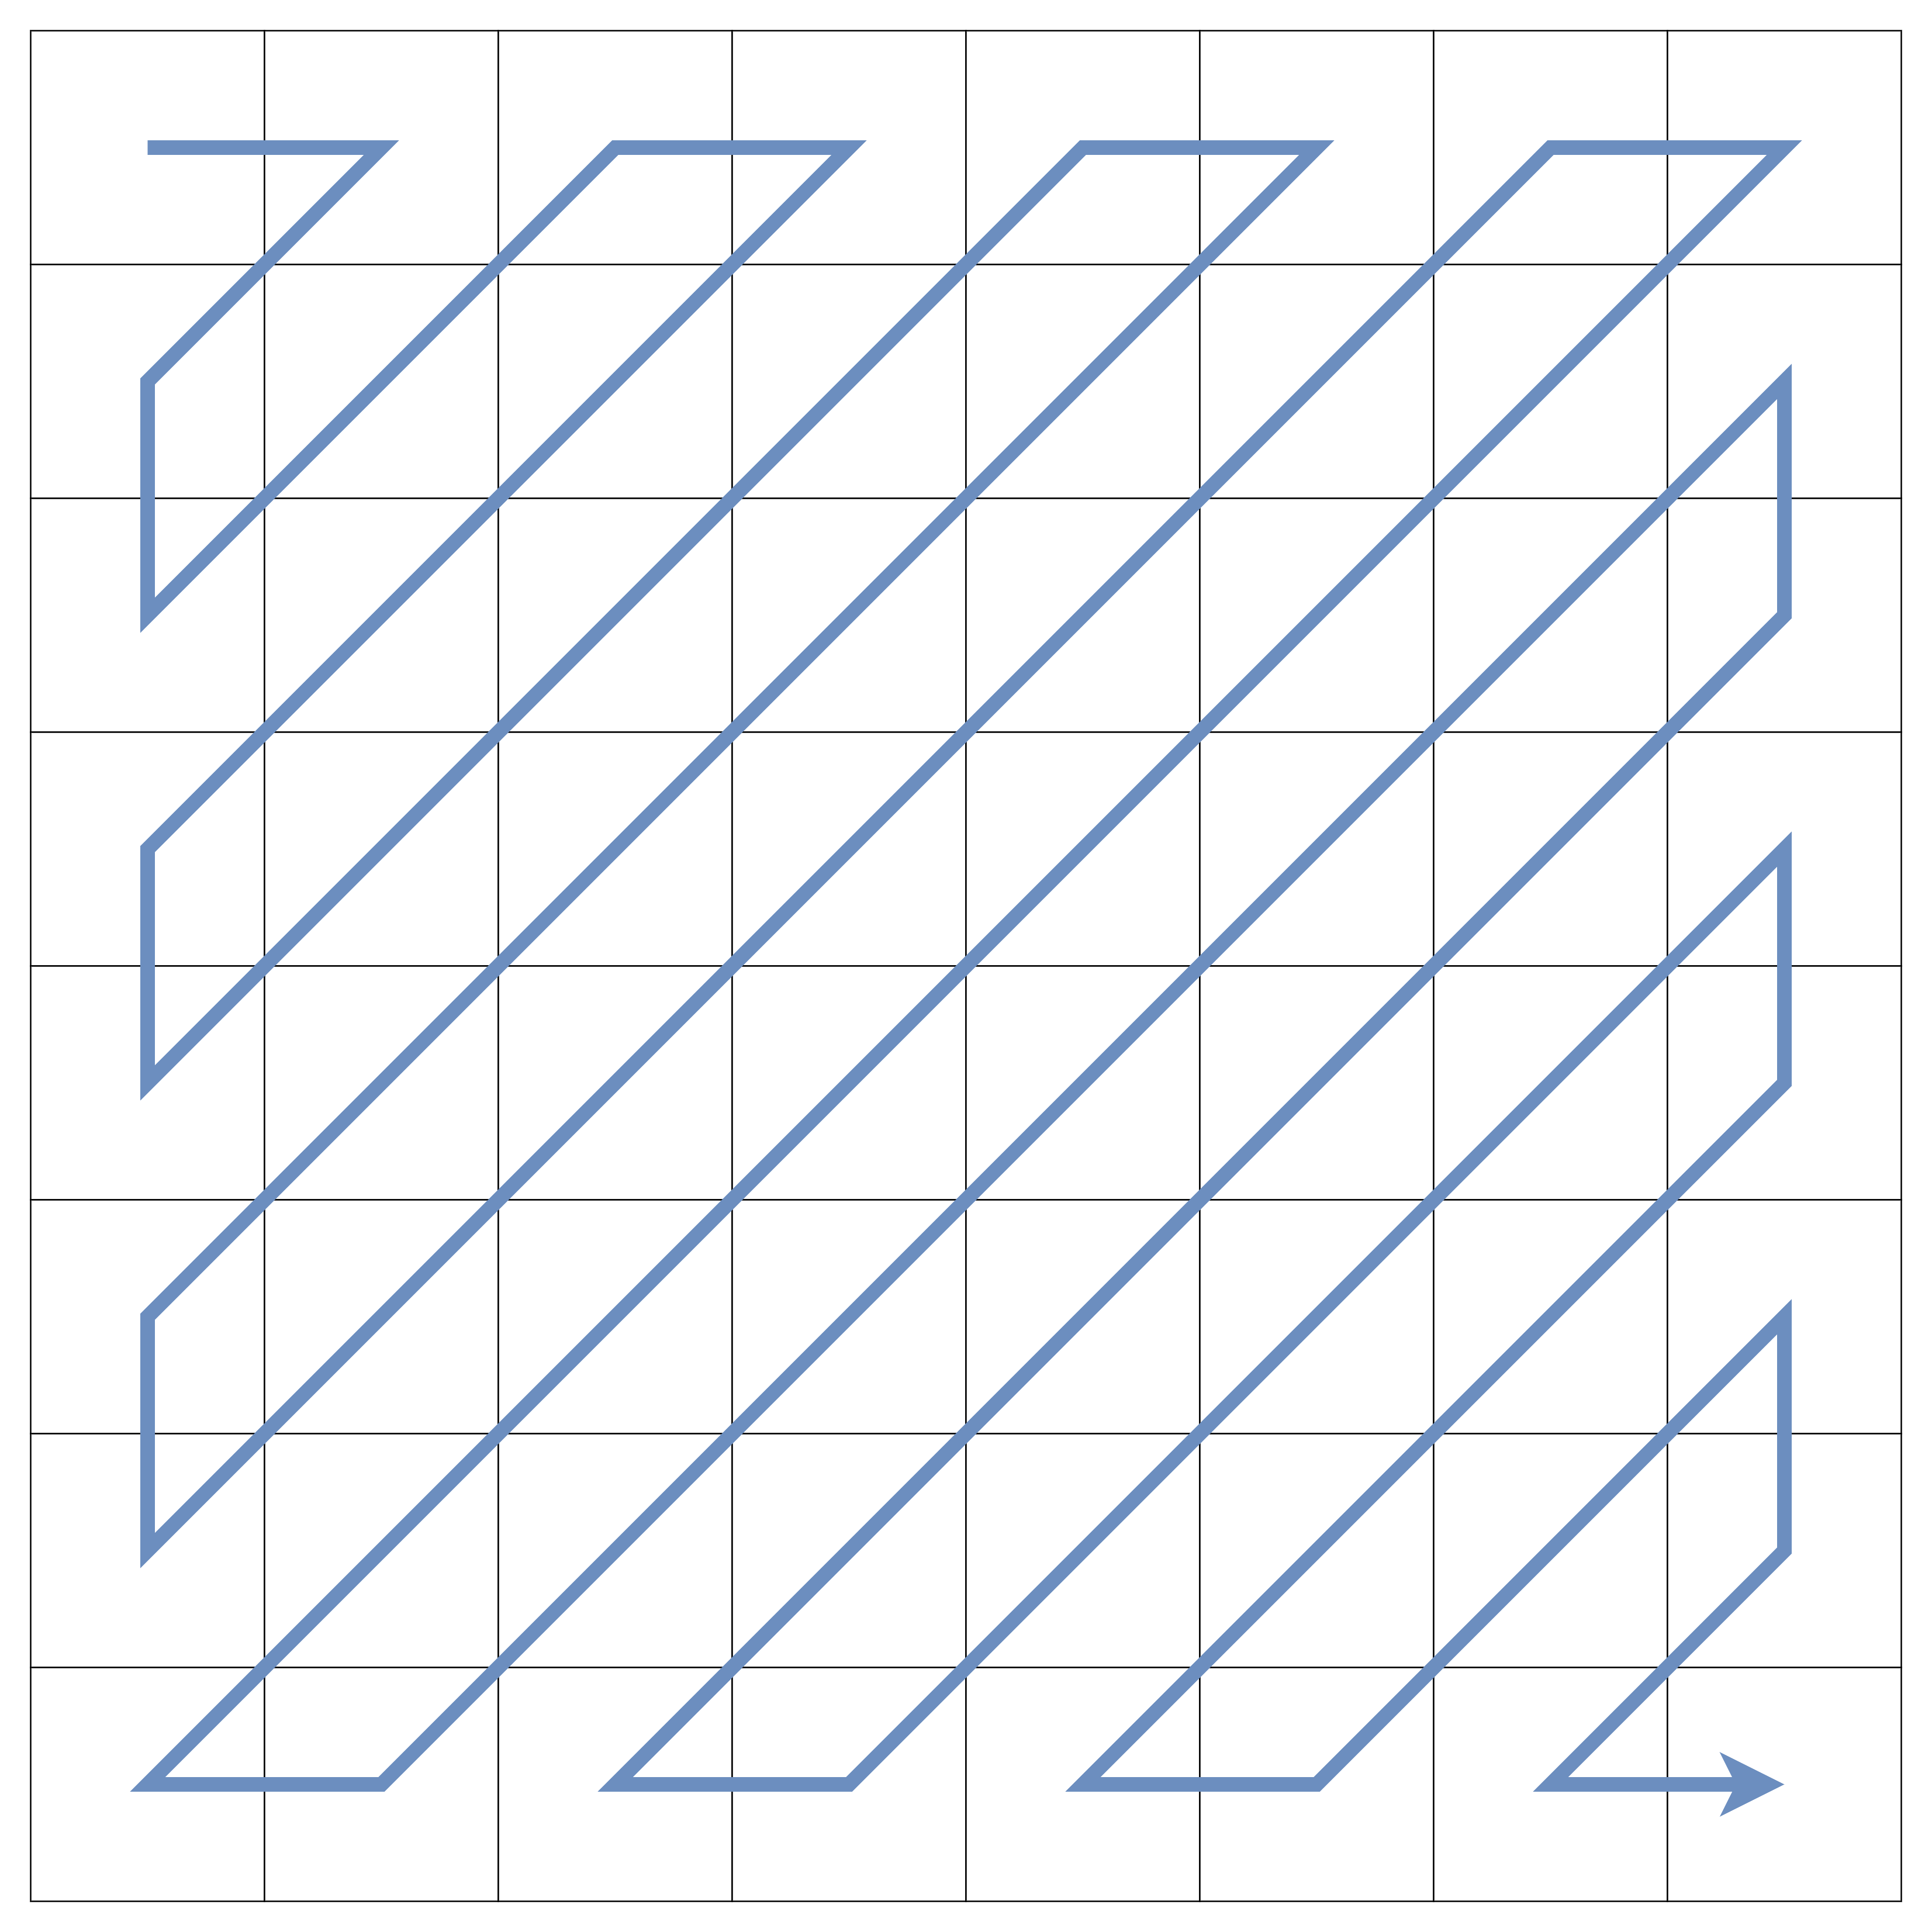
\includegraphics[width=10cm]{./images/zigzag-order.png}
    \caption{Порядок сканирования коэффициентов ДКП}
    \label{image:zigzag-order}
\end{figure}

Множество различных пар $(run,\ level)$ представляет собой дискретный ансамбль~\cite{information-theory} --- некоторое множество $X$, в котором каждому элементу $x\in X$ приписана вероятность $p(x)$, определяемая частотой, с которой данная пара встречается в компоненте изображения, что соответствует собственной информации $I(x)=-\log p(x)$. Эффективность побуквенного кодирования компонента определяется его энтропией --- величиной $\mathbb{E}(-\log p(x))=-\sum_{x\in X}p(x)\log p(x)$. Чем ниже энтропия, тем более эффективно побуквенное кодирование, а оптимальным побуквенным кодом является код Хаффмана, основанный на идее о том, что пары $(run, level)$ с более высокими вероятностями (содержащие меньшее значение собственной информации) должны иметь более короткие коды. Именно такой способ кодирования применяется в алгоритме JPEG. Каждая пара $(run,\ level)$ кодируется кодом Хаффмана, а следом за ней в выходящий битовый поток записывается двоичное представление коэффициента ДКП в прямом коде.\par

Необходимо отметить, что способ построения таблицы Хаффмана при кодировании алгоритмом JPEG не задан стандартом. При практической реализации применяется один из двух подходов:
\begin{enumerate}
    \item Однопроходный, при котором используются универсальные таблицы Хаффмана, содержащие в себе кодовые слова для всех возможных пар $(run,\ level)$;
    \item Двухпроходный, при котором таблицы Хаффмана строятся для конкретного изображения.
\end{enumerate}

\section{Эффективные методы сжатия изображений}\label{sec:effective-compression-methods}

На сегодняшний день в области сжатия изображений есть большие успехи. Так, например, следующие форматы позволяют достичь гораздо большей степени сжатия c потерями при заданном качестве картинки~\cite{mozilla-comparison-of-compression-formats}:
\begin{enumerate}
    \item JPEG2000~\cite{jpeg2000-overview} --- алгоритм, аналогичный JPEG, но основанный на вейвлет-преобразовании (альтернативном методе преобразования сигналов (изображений) из пространства времени (пикселей) в пространство частот) и арифметическом кодировании;
    \item BPG (Better Portable Graphics)~\cite{bpg-website} --- алгоритм основанный на видеокодеке HEVC (технологии кодирования ключевых кадров). В нем изображение делится на блоки разного, а не фиксированного (в отличие от JPEG) размера. Данный формат поддерживает сжатие с потерями и без, изображение с альфа-каналом (прозрачностью), использование метаданных и анимацию;
    \item WebP (WEB Pictures)~\cite{webp-overview} --- алгоритм, аналогичный по функциональности BPG, но основанный на видеокодеке VP8. Изображение, закодированное данным форматом на 25--34\% меньше, чем идентичное по качеству JPEG-изображение.
\end{enumerate}

Однако вышеперечисленные форматы не используются так широко, как JPEG, из-за своей высокой вычислительной сложности. Между тем существует ряд алгоритмов сжатия без потерь, например:

\begin{enumerate}
    \item JPEG-LS~\cite{jpeg-ls-overview} --- формат сжатия, представленный Joint Photographic Experts Group в дополнение к JPEG и JPEG2000, но ориентированный именно на сжатие без потерь. Реализует адаптивное предсказание значений пикселей по уже закодированным значениям, а также  классификацию контекста, контекстное моделирование ошибки предсказания и её коррекцию. В качестве энтропийного кодирования ошибок предсказания применяются коды Голомба;
    \item CALIC (context-based, adaptive, lossless image codec)~\cite{calic-overview} --- алгоритм, использующий большое число контекстов моделирования для нелинейного предиктора и его адаптации к изменяющейся статистике источника;
    \item FLIF (Free Lossless Image Format)~\cite{flif-website} --- формат, который по заверениям разработчиков превосходит по эффективности сжатия все перечисленные форматы. Данный метод использует вариацию арифметического кодирования в качестве энтропийного сжатия.
\end{enumerate}

К сожалению, все они являются неэффективными для транскодирования JPEG-изображений без потерь. Связано это, в частности, с округлением значений Y, Cb, Cr и коэффициентов ДКП при кодировании и ограничении значений R, G, B при декодировании, о чем будет упомянуто ниже, в разделе~\ref{subsec:common-methods}. Несмотря на это, необходимо обратить внимание на то, что все эти подходы:
\begin{enumerate}
    \item Реализуют более сложные методы внутреннего предсказания, чем алгоритм JPEG, так как основаны на пространственной корреляции, наблюдаемой между соседними участками изображений;
    \item Используют более эффективные, чем код Хаффмана, подходы для энтропийного кодирования ошибок предсказания.
\end{enumerate}

\section{Транскодирование JPEG-изображений с потерями}\label{sec:lossy-transcoding-overview}

Возможность дополнительного сжатия именно JPEG-изображений выглядит привлекательной, причем это может быть как транскодирование с потерями, так и без. Первую задачу успешно выполняют такие программы как:
\begin{enumerate}
    \item TinyPNG~\cite{tinypng-project}, достигающий высокой степени сжатия за счет объединения цветов, изменения порядка сканирования и использования особенностей человеческого зрения;
    \item Mozjpeg~\cite{mozjpeg-github-page}, являющийся эффективным кодером JPEG от компании Mozilla и реализующий возможность транскодирования JPEG, закодированных другим кодером, в более эффективное представление;
    \item Guetzli~\cite{guetzli-overview}, также является эффективным кодером JPEG, но от компании Google.
\end{enumerate}

Несмотря на успехи в области сжатия с потерями, во многих прикладных сценариях сжатие оно недопустимо. Примером таких задач может быть хранение данных пользователя в облачных хранилищах.

\section{Транскодирование JPEG-изображений без потерь}\label{sec:lossless-transcoding-overview}

Утилиты, реализующие транскодирование без потерь, также существуют. Наиболее ранней и распространенной является Jpegtran~\cite{jpegtran-description, jpegtran-project}, которая, однако, далека от предела возможностей современных транскодеров, таких как LLJPEG~\cite{lljpeg-overview, lljpeg-testing}. В данном разделе рассмотрены общие подходы к транскодированию изображений и упомянутые программы, выполняющие транскодирование файлов JPEG без потерь.

\subsection{Общие методы}\label{subsec:common-methods}

Общие положения, лежащие в основе любого транскодера JPEG, были выдвинуты авторами Jpegtran еще в 2005 году~\cite{jpegtran-description}. Основаны они на том факте, что при декодировании и повторном кодировании JPEG файла результат может быть отличным от исходного даже при фиксированном значении параметра $QF$. Рассмотрим более подробно, откуда возникают неконтролируемые потери.\par

Первыми этапами при декодировании JPEG-файлов являются применение энтропийного декодера (кода Хаффмана) и обратное квантование. На данных этапах не может возникать никаких дополнительных потерь. Далее выполняется обратное ДКП и на практике эта операция не является обратимой, так как после применения ДКП в алгоритме JPEG коэффициенты округляются до целых чисел. К тому же в зависимости от деталей реализации вычислений, методов округления могут возникать незначительные с точки зрения качества изображения, но не кодирования информации ошибки. Это же относится и к преобразованию цветового пространства.\par

Так, например, функция преобразования YCbCr в RGB может возвращать дробные, отрицательные значения или значения больше 255, иными словами --- некорректные значения пикселей в RGB. Для устранения этих ошибок применяется округление до целого и функция
\begin{equation*}
    clip(x)=\begin{cases}
        0,   & x < 0,     \\
        255, & x > 255,   \\
        x,   & otherwise.
    \end{cases}
\end{equation*}

Таким образом, для транскодирования JPEG-изображений без потерь можно выполнять модификации алгоритма на этапах, следующих за ДКП --- устранять избыточность между коэффициентами преобразования благодаря реализации механизмов внутреннего предсказания, а также дорабатывать этап энтропийного кодирования.

\subsection{Jpegtran}\label{subsec:jpegtran}

Утилита Jpegtran была разработана в 2005 году и предназначалась в первую очередь для выполнения преобразований над JPEG-изображениями без потерь. Так, например, она поддерживает такие функции, как поворот (rotate), отражение (flip), транспонирование (transpose) и другие. Их выполнение возможно с помощью применения аналогичных преобразований над блоками изображения, таблицами квантования и т.д. Подобные трансформации приводят к изменению размеров файлов JPEG, причем как в большую, так и в меньшую сторону. Происходит это благодаря тому, что после выполнения каких-либо преобразований на вход энтропийному кодеру поступает отличная от исходной последовательность кодовых слов --- пар $(run,\ level)$. Фактически, возможность транскодирования JPEG-изображений с целью дополнительного сжатия --- это удобный побочный эффект утилиты Jpegtran.\par

Более современные версии Jpegtran поддерживают также ряд преобразований, направленных именно на дополнительное сжатие (транскодирование) JPEG-изображений без потерь:
\begin{enumerate}
    \item Опция \texttt{-optimize} позволяет выполнять оптимизацию таблицы Хаффмана под конкретное изображение. Как было упомянуто в разделе~\ref{subsec:entropy-coding}, для ускорения кодирования JPEG могут использоваться универсальные таблицы Хаффмана, содержащие кодовые слова для любых возмножных пар $(run,\ level)$. Поскольку распределение вероятностей конкретного изображения может отличаться от универсального, для него может быть более эффективный код;
    \item Опция \texttt{-arithmetic} позволяет заменить код Хаффмана на арифметическое кодирование.
\end{enumerate}

\subsection{LLJPEG}\label{subsec:lljpeg}

Разработанный в 2023 году LLJPEG является одним из наиболее эффективных решений задачи о транскодировании файлов JPEG без потерь. Данный метод --- это гибридный алгоритм, объединяющий сразу несколько эффективных подходов к транскодированию JPEG-изображений:
\begin{enumerate}
    \item При делении на блоки используется адаптивный размер, который итеративно вычисляется для каждого участка изображения. Начиная со значения $64\times64$, на каждой итерации рассчитывается стоимость кодирования блока и, пока это является эффективным, --- блок уменьшается. Минимальный допустимый размер блока --- $4\times4$;
    \item В качестве метода внутреннего предсказания используется подход аналогичный внутреннему предсказанию видеокодека HEVC, где для вычисления значений в блоке используется наиболее эффективное направление из 35-и, указывающих на блоки слева и сверху. Необходимо отметить, что возможности такого подхода ограничены, так как для предсказания используется только локальная схожесть, наблюдаемая в изображении, но не учитывается подобие удаленных друг от друга участков. Если же учесть нелокальную схожесть пикселей, то гипотетически можно добиться более эффективного предсказания и, следовательно, устранения избыточности.
    \item Код Хаффмана заменяется более эффективным контекстно-адаптивным бинарным арифметическим кодером (context-adaptive binary arithmetic coding, CABAC).
\end{enumerate}

Благодаря объединению вышеперечисленных техник эффективность сжатия LLJPEG достигает порядка $18\%$ для параметра $QF=90$, что на сегодняшний день является наилучшим показателем.

\chapterconclusion

В данной главе были подробно рассмотрены основные этапы работы алгоритма JPEG, а также проведен обзор других, более эффективных, методов сжатия изображений с потерями и без, появившихся уже после широкого распространения JPEG. Длаее были рассмотрены методы транскодирования изображений с потерями: TinyPNG, Mozjpeg, Guetzli. И наконец, был проведен анализ литературы на тему того, за счет чего может выполняться транскодирование и как эти подходы реализованы в существующих решениях: Jpegtran и LLJPEG. В результате было показано, что все соверменные алгоритмы сжатия изображений, позволяющие достигать более высокой степени сжатия, чем JPEG, а также методы транскодирования без потерь основаны на улучшении двух важных этапов: внутреннего предсказания коэффициентов ДКП и энтропийного кодирования. Второй из этих пунктов практически всегда подразумевает использование различных вариаций адаптивного арифметического кодирования, а первый в большинстве эффективных алгоритмов заимствован из видеокодека HEVC.

\finishrelatedwork

\chapter{Транскодирование JPEG-изображений на основе нейросетевого внутреннего предсказания}\label{chapter:neural-network-transcoder}

В данной главе описывается предалагаемый алгоритм транскодирования JPEG-изображений, основанный на нейросетевом внутреннем предсказании.

\section{Мотивация}\label{section:motivation}

Как было упомянуто в разделе~\ref{subsec:common-methods}. Эффективность сжатия зависит от нескольких факторов. С одной стороны, можно оптимизировать энтропийный кодер. Например, строить оптимальные таблицы Хаффмана для конкретного изображения двухпроходным алгоритмом, а не использовать универсальные, либо вовсе отказываться от кода Хаффмана в пользу арифметического кодирования. Кроме того, внутреннее предсказание позволяет уменьшать число ненулевых коэффициентов и их абсолютные значения. Это также положительно сказывается на степени сжатия, так как серии из нулей кодируются эффективно благодаря применению RLE, а меньшим по модулю коэффициентам обычно соответствуют более короткие кодовые слова.\par

В разделе~\ref{sec:lossless-transcoding-overview} упоминалось, что задача внутреннего предсказания коэффициентов ДКП уже решается с использованием простых конечных алгоритмов, например, в видеокодеках VVC и HEVC, а также в LLJPEG (в последних двух случаях используются одинаковые подходы). Суть данных алгоритмов состоит в поиске зависимостей между кодируемым блоком и одним или несколькими соседними блоками из того же компонента. На рисунке~\ref{image:hevc-intra-prediction} показано, как реализуется внутреннее предсказание в видеокодеке HEVC, а на рисунке~\ref{image:planar-inta-rediction} --- пример применения планарного (planar) режима предсказания. Из приведенного примера видно, что внутреннее предсказание не учитывает нелокальную схожесть разных участков изображения.\par

\begin{figure}[!h]
    \centering
    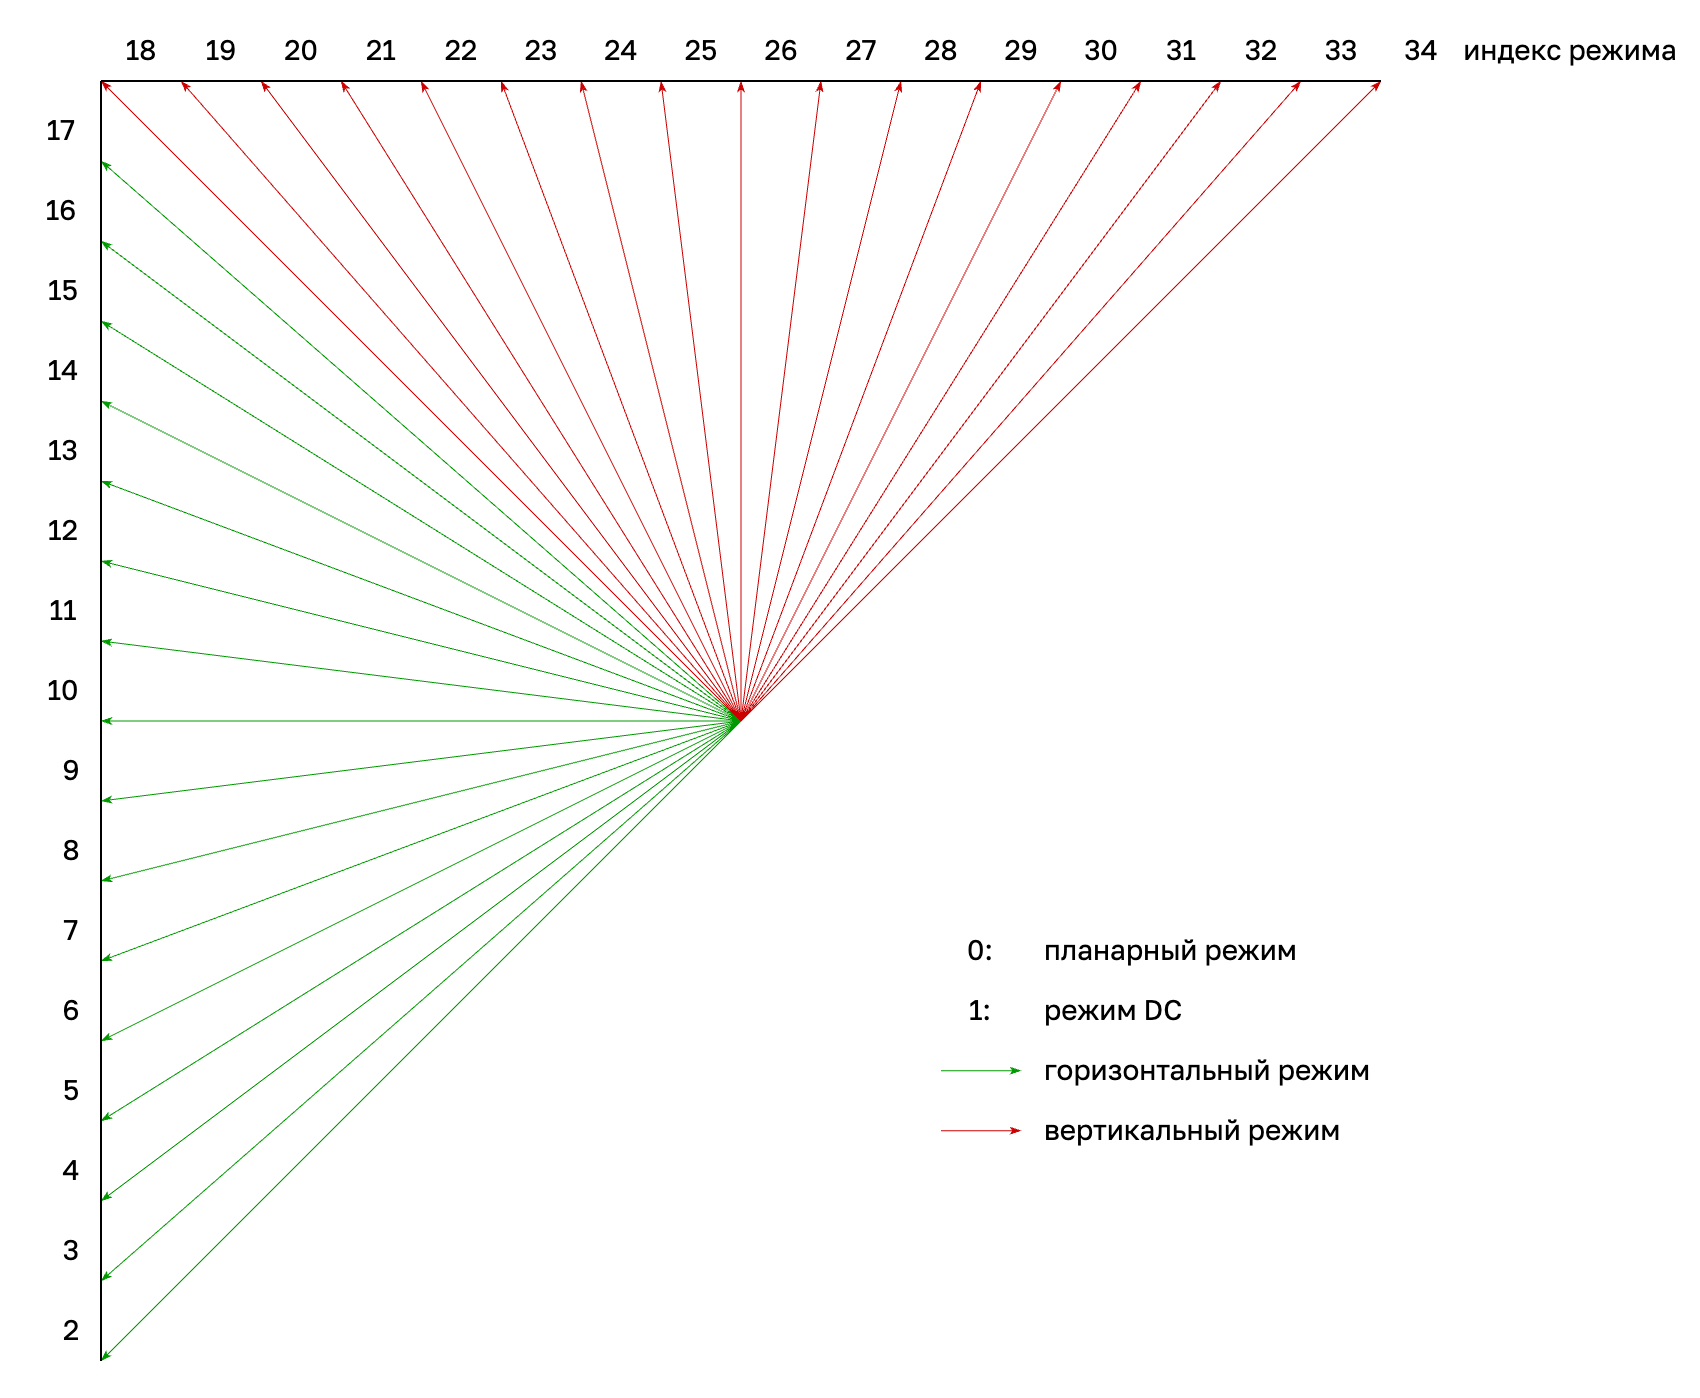
\includegraphics[width=12cm]{./images/hevc-intra-prediction.png}
    \caption{Режимы внутреннего предсказания в видеокодеке HEVC; красные и зеленые линии представляют вертикальные и горизонтальные режимы; режим 0 - это планарный (planar) режим; а режим 1 - режим DC}
    \label{image:hevc-intra-prediction}
\end{figure}

\begin{figure}[!h]
    \centering
    
\includegraphics[width=6cm]{./images/planar-inta-rediction.png}
    \caption{Планарный (planar) режим внутреннего предсказания в видеокодеке HEVC}
    \label{image:planar-inta-rediction}
\end{figure}

В основе настоящей работы лежит идея о том, что для предсказания коэффициентов ДКП можно использовать нейронную сеть. Преимущество данного подхода по сравнению с уже существующими заключается в том, что модели машинного обучения способны искать более сложные взаимосвязи в изображении, например:
\begin{itemize}
    \item между блоком изображения и его соседями (в любом из направлений);
    \item между яркостным (Y) и цветовыми (Cr, Cb) компонентами;
    \item между удаленными друг от друга участками изображения.
\end{itemize}

Таким образом, основную гипотезу можно сформулировать следующим образом: эффективность внутреннего предсказания на основе нейронной сети может превышать эффективность подходов, использующих локальные зависимости между соседними блоками.

\section{Обзор предлагаемого алгоритма}\label{section:algorithm-overview}

В настоящей работе предлагается новый метод предсказания коэффициентов ДКП и алгоритм транскодирования JPEG-изображений, основанный на данном подходе.

\subsection{Транскодирование}\label{subsection:transcoding-overview}

На рисунке~\ref{encoder-scheme} представлена общая схема транскодера.

\begin{figure}[!h]
    \centering
    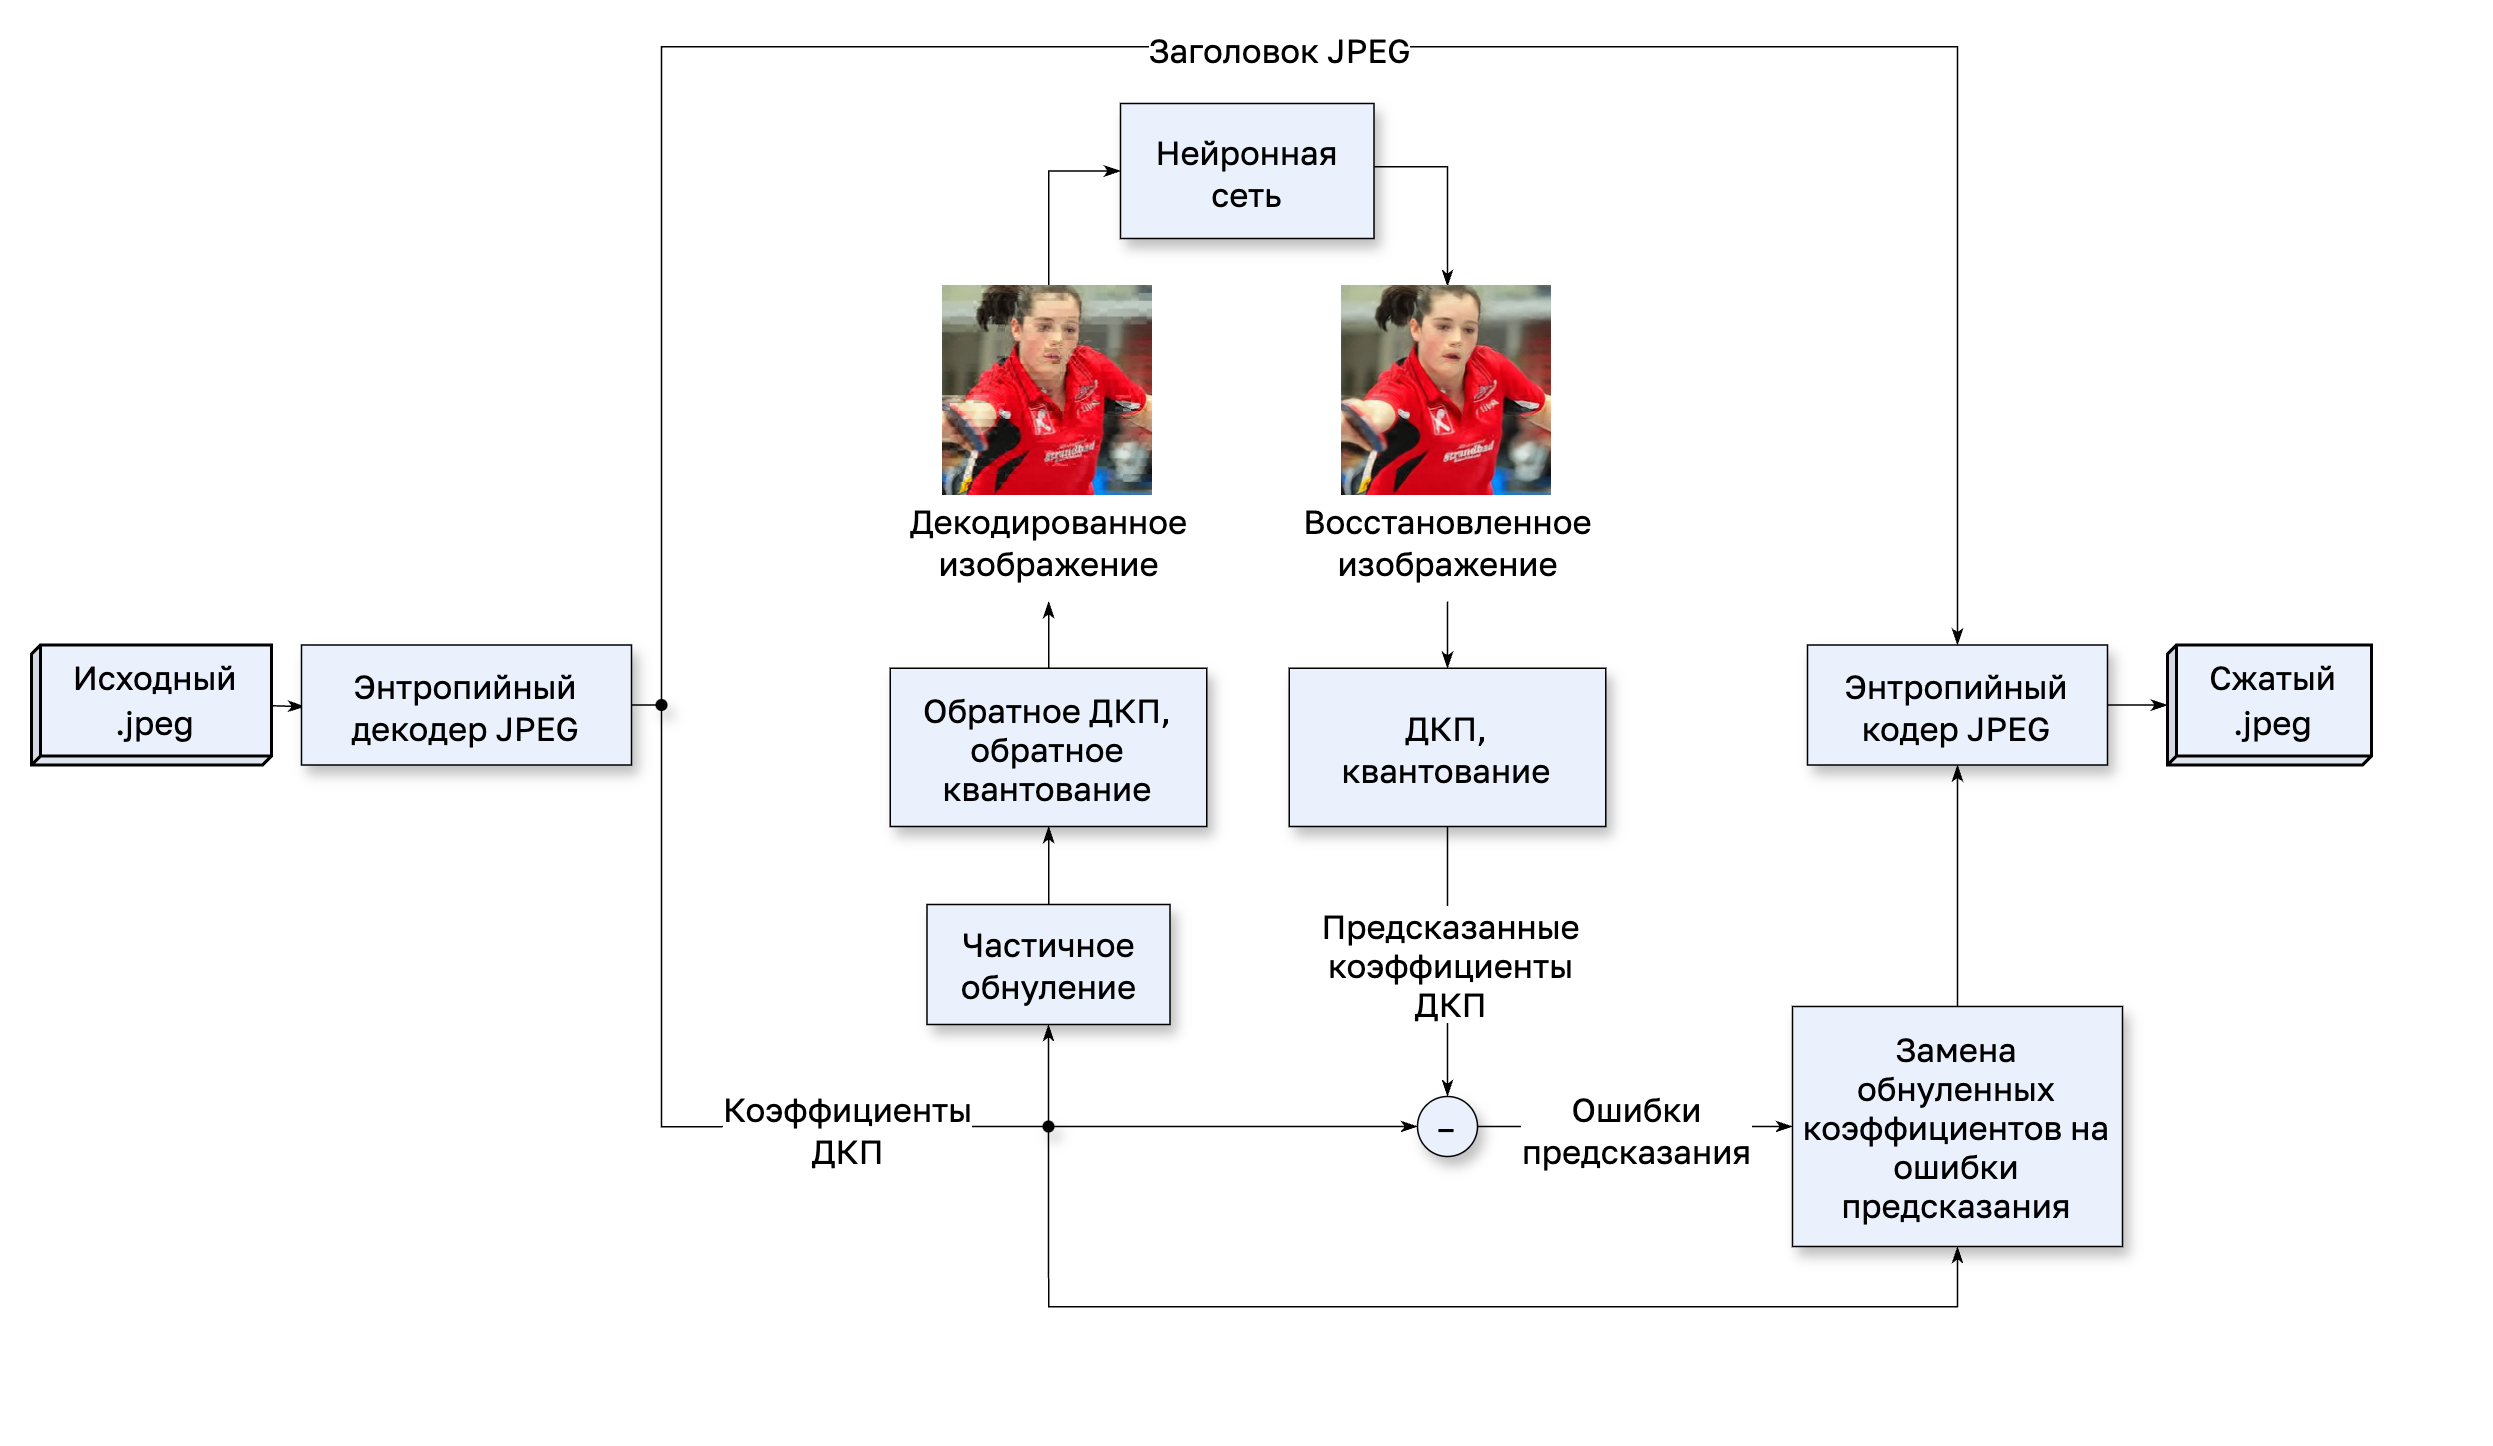
\includegraphics[width=\textwidth]{./images/encoder-scheme.png}
    \caption{Общая схема работы транскодера}
    \label{encoder-scheme}
\end{figure}

При транскодировании к исходному изображению $I$ применяется энтропийный декодер JPEG, а затем из него извлекаются квантованные коэффициенты ДКП. Далее они делятся псевдослучайным образом на две группы и коэффициенты первой группы обнуляются. Пример такого преобразования представлен на рисунке~\ref{image:block-transformation-example}~(б).\par

\begin{figure}[!h]
    \centering
    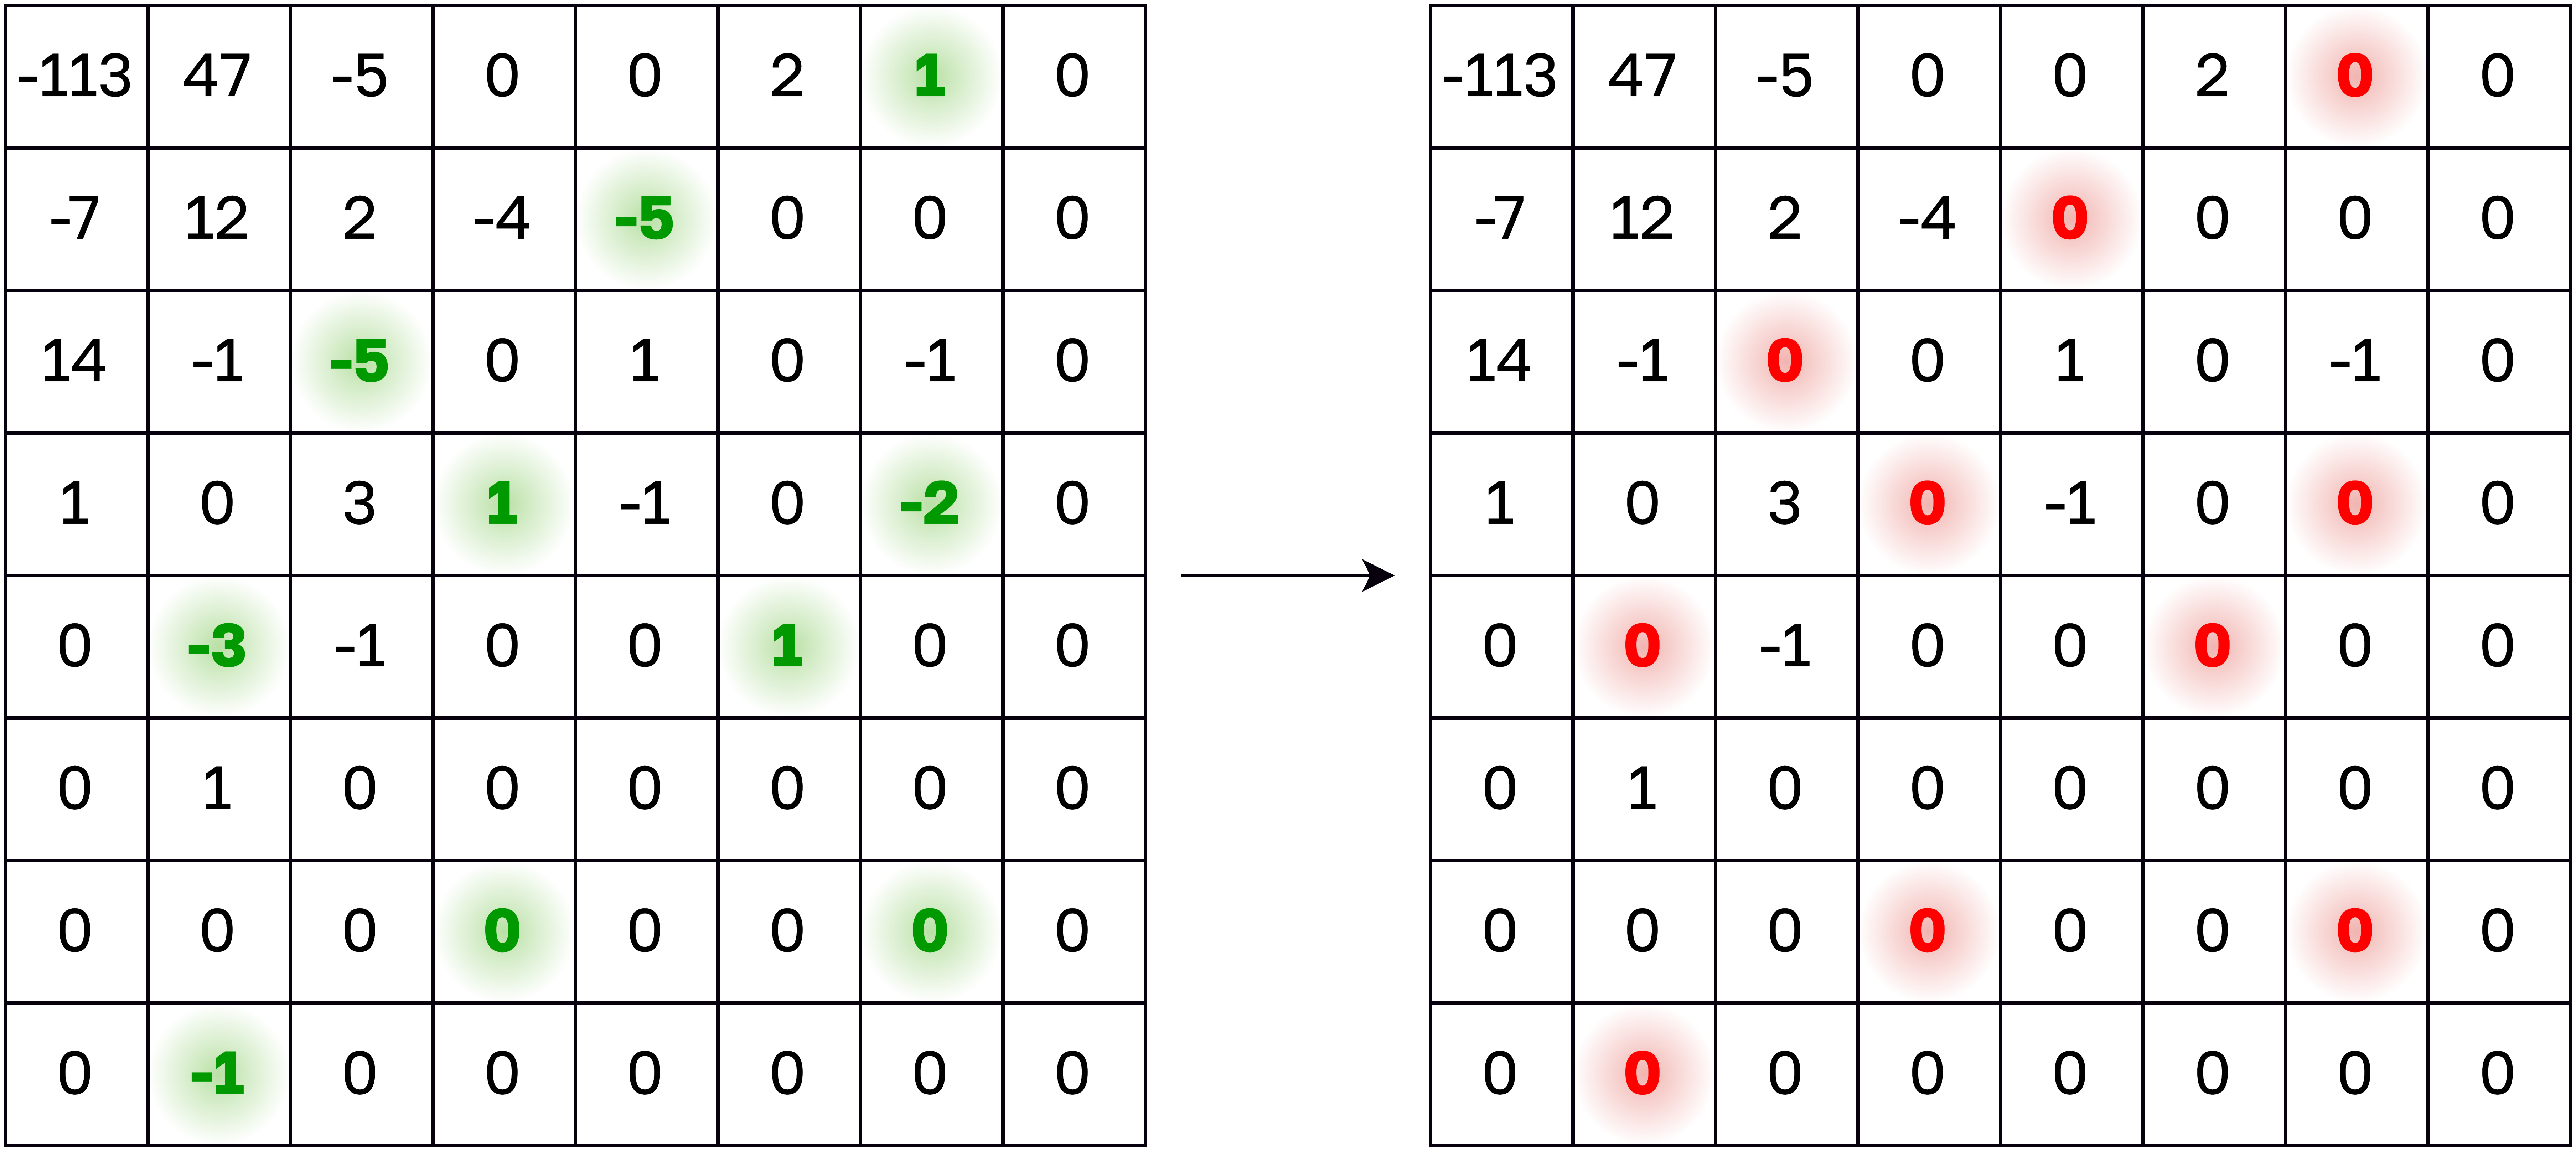
\includegraphics[width=13cm]{./images/block-transformation-example.png}
    \caption{Пример преобразований над блоком: а) исходный блок; б) блок после обнуления части коэффициентов; в) блок на выходе нейронной сети; г) блок с ошибками предсказания на местах исходных коэффициентов}
    \label{image:block-transformation-example}
\end{figure}

После обнуления блока к оставшимся коэффициентам применяется обратное квантование и обратное ДКП, и изображение переводится в цветовое пространство RGB. Таким образом, фактически выполняется стандартное декодирование JPEG, но изображение оказывается искаженным ($\tilde{I}$). Далее оно подается на вход нейронной сети $M$, которая обучена улучшать качество декодированных изображений. В области ДКП это означает, что на местах обнуленных коэффициентов $x_{i,j}$ первой группы в обработанном моделью изображении $I'=M(\tilde{I})$ появляются похожие на них коэффициенты $x'_{i,j}$ (рисунок~\ref{image:block-transformation-example}~(в)). Таким образом, нейронная сеть предсказывает значения коэффициентов первой группы по коэффициентам из второй группы, то есть реализует внутреннее предсказание.\par

На следующем этапе все коэффициенты кодируются согласно алгоритму JPEG, однако вместо значений коэффициентов первой группы кодируется ошибка их предсказания $\Delta x_{i,j}=x_{i,j}-x'_{i,j}$. Если нейронной сети удается в точности восстанновить обнуленный коэффициент ($x'_{i,j}=x_{i,j}$), то вместо него в блоке остается ноль, в противном случае коэффициент заменяется меньшим по модулю значением. Таким образом, достигается дополнительное сжатие JPEG-изображения.\par

\subsection{Трансдекодирование}\label{subsection:transdecoding-overview}

Схема трансдекодера представлена на рисунке~\ref{decoder-scheme} и аналогична схеме транскодера. При декодировании создается изображение $\tilde{I}$, у которого удалены те же самые коэффициенты, что и при кодировании. Оно подается на вход нейронной сети $M$ и на месте обнуленных коэффициентов появляются значения $x'$, к которым остается только добавить поправку $\Delta x$, закодированную на местах удаленных коэффициентов. В результате получаются $x = x' + \Delta x$ --- исходные значения коэффициентов ДКП, которые далее кодируются энтропийным кодером JPEG.

\begin{figure}[!h]
    \centering
    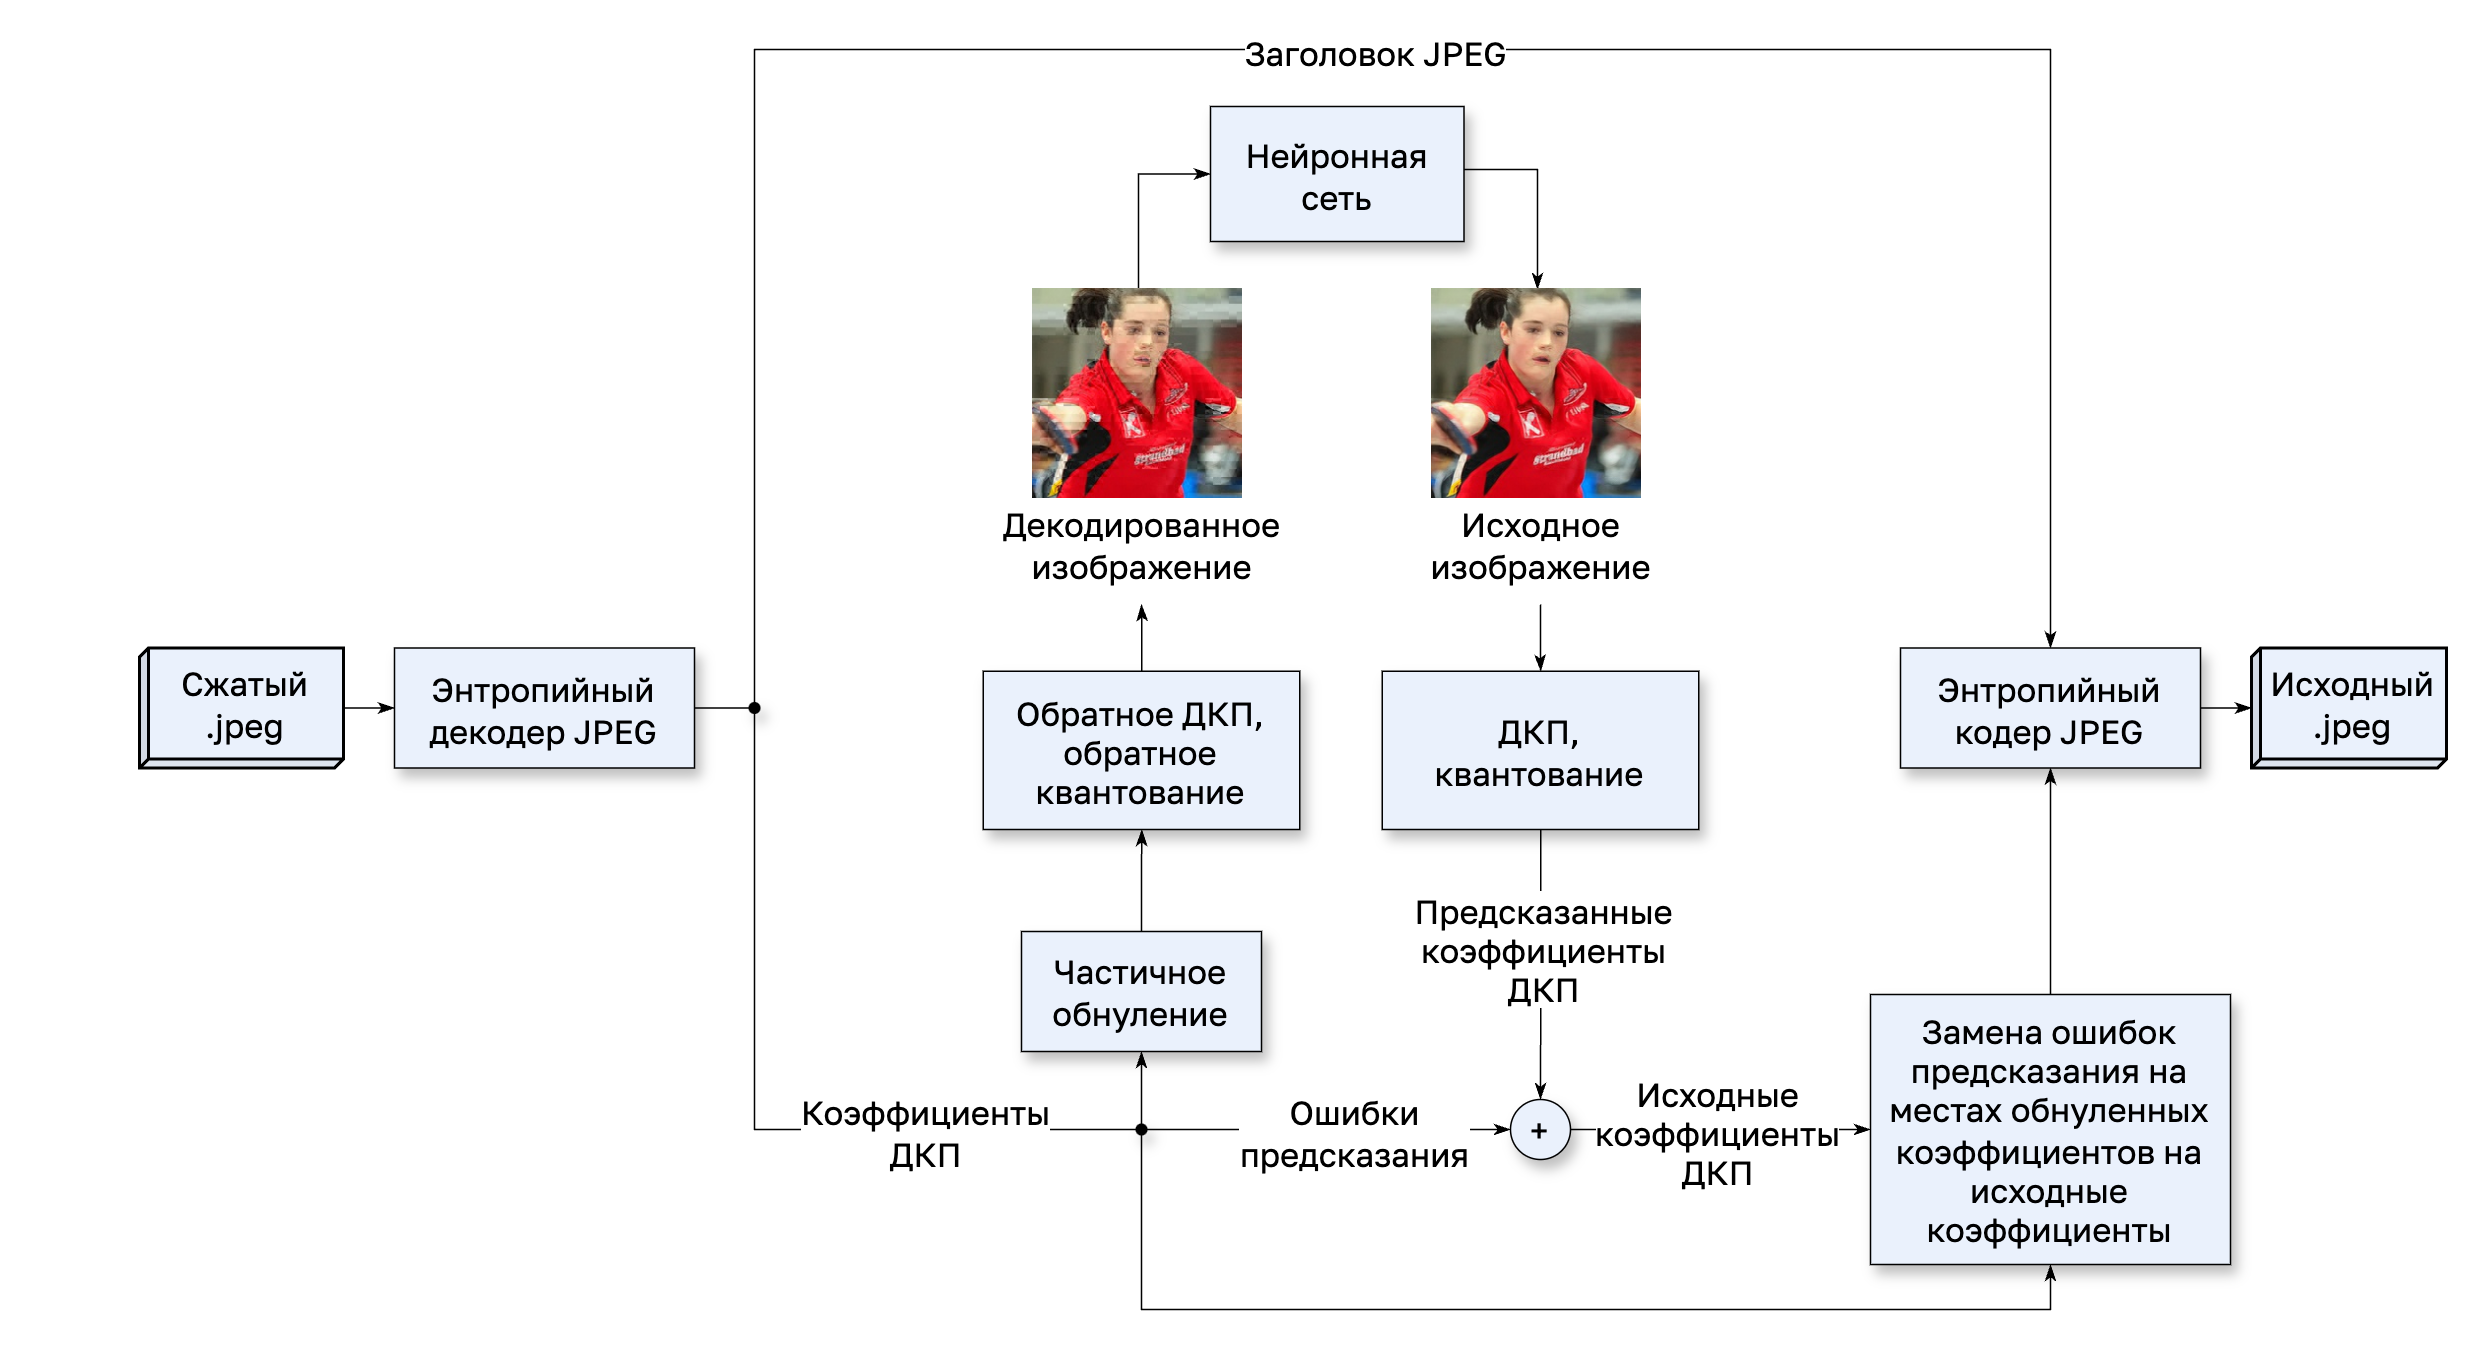
\includegraphics[width=\textwidth]{./images/decoder-scheme.png}
    \caption{Общая схема работы трансдекодера}
    \label{decoder-scheme}
\end{figure}

\section{Обнуление коэффициентов}\label{section:zeroing-the-coefficients}

Обнуление коэффициентов является одним из ключевых этапов транскодирования. К нему выдвигаются следующие требования:
\begin{enumerate}
    \item \textit{Детерминированность}. Список обнуленных коэффициентов должен быть известен при декодировании, а значит, независимо от изображения он должен быть определен;
    \item \textit{Псевдослучайность}. В соседних блоках должны удаляться совершенно разные коэффициенты (настолько, насколько это возможно), так как если наборы обнуляемых коэффициентов существенно отличаются друг от друга, их восстановление может происходить благодаря заимствованию информации из соседних блоков.
\end{enumerate}

Необходимо также отметить тот факт, что стандарт JPEG подразумевает существенное сокращение вклада цветовых компонентов в итоговый объем файла благодаря прореживанию. В то же время, яркостный компонент кодируется в исходном виде. Следовательно, наибольшее преимущество описанного способа кодирования следует ждать в случае применения его к компоненту Y. Каналы Cb и Cr, напротив, могут быть использованы нейронной сетью для восстановления изображения благодаря тому, что между яркостным и цветовыми компонентами существует локальная пространственная корреляция.

\section{Внутреннее предсказание коэффициентов}\label{section:intra-prediction}

Для улучшения качества закодированных изображений обычно используются сверточные нейронные сети. В данном разделе рассматриваются архитектуры моделей машинного обучения, позволяющие решить данную задачу, а также функции потерь, подходящие для обучения этих моделей.

\subsection{AR-CNN}\label{subsection:ar-cnn}

Архитектура AR-CNN (Artifacts Reduction Convolutional Neural Network)~\cite{ar-cnn-overview} призвана устранять артефакты, возникающие на изображении при кодировании его алгоритмом JPEG. Архитектура данной сети содержит три сверточных слоя, между которыми применяется функция-активации $ReLU$. Математически ее можно описать следующим образом:
\[
    ReLU(x) = \max(0, x),
\]
\[
    F_0(Y) = Y,
\]
\[
    F_i(Y) = ReLU(W_i * F_{i-1}(Y) + B_i),\quad i \in \{1, 2\},
\]
\[
    F(Y) = W_3 * F_2(Y) + B_3,
\]
где $W_i$ и $B_i$ --- это веса сверточных фильтров и сдвиги $i$-го слоя соответственно, $F_i$ --- значения на выходе сверточных слоев, а <<$*$>> означает операцию свертки.\par

Результаты экспериментов показывают, что данная архитектура действительно хорошо устраняет искажения, вызванные работой JPEG, однако не справляется с более сложными артефактами, появляющимися, например, после работы других методов кодирования изображений и видео. Исследования показывают, что причиной этому является недостаточное количество сверточных слоев.

\subsection{QE-CNN-P}\label{subsection:qe-cnn}

На базе AR-CNN была разработана архитектура QE-CNN-P (Quality Enhancement Convolutional Neural Network)~\cite{qe-cnn-overview}, имеющая больше сверточных слоев, но способная искать более сложные искажения и устранять их. Именно данную архитектуру предлагается использовать для реализации внутреннего предсказания в транскодере JPEG-изображений. Она представленна на рисунке~\ref{model-architecture}. Каждый ее слой состоит из свертки, сохраняющей размерность тензора, и функции активации $PReLU$ с числом параметров равном числу фильтров в свертке. Математически данная архитектура может быть выражена следующим образом:
\[
    PReLU_i(x) = \max(0, x) + a_i \cdot \min(0, x),
\]
\[
    F_0(Y) = Y,
\]
\[
    F_i(Y) = PReLU_i(W_i * F_{i-1}(Y) + B_i),\quad i \in \{1, 2, 3, 4\},
\]
\[
    F_5(Y) = PReLU_5(W_5 * F_0(Y) + B_5),
\]
\[
    F_i(Y) = PReLU_i(W_i * (F_{i-5}(Y) \oplus F_{i-1}(Y)) + B_i),\quad i \in \{6, 7, 8\},
\]
\[
    F_9(Y) = W_9 * (F_4(Y) \oplus F_8(Y)) + B_9,
\]
где $a_i$ --- обучаемый параметр функции активации $ReLU_i$, представляющий из себя вектор значений, а <<$\oplus$>> означает конкатенацию тензоров.\par

\begin{figure}[!h]
    \centering
    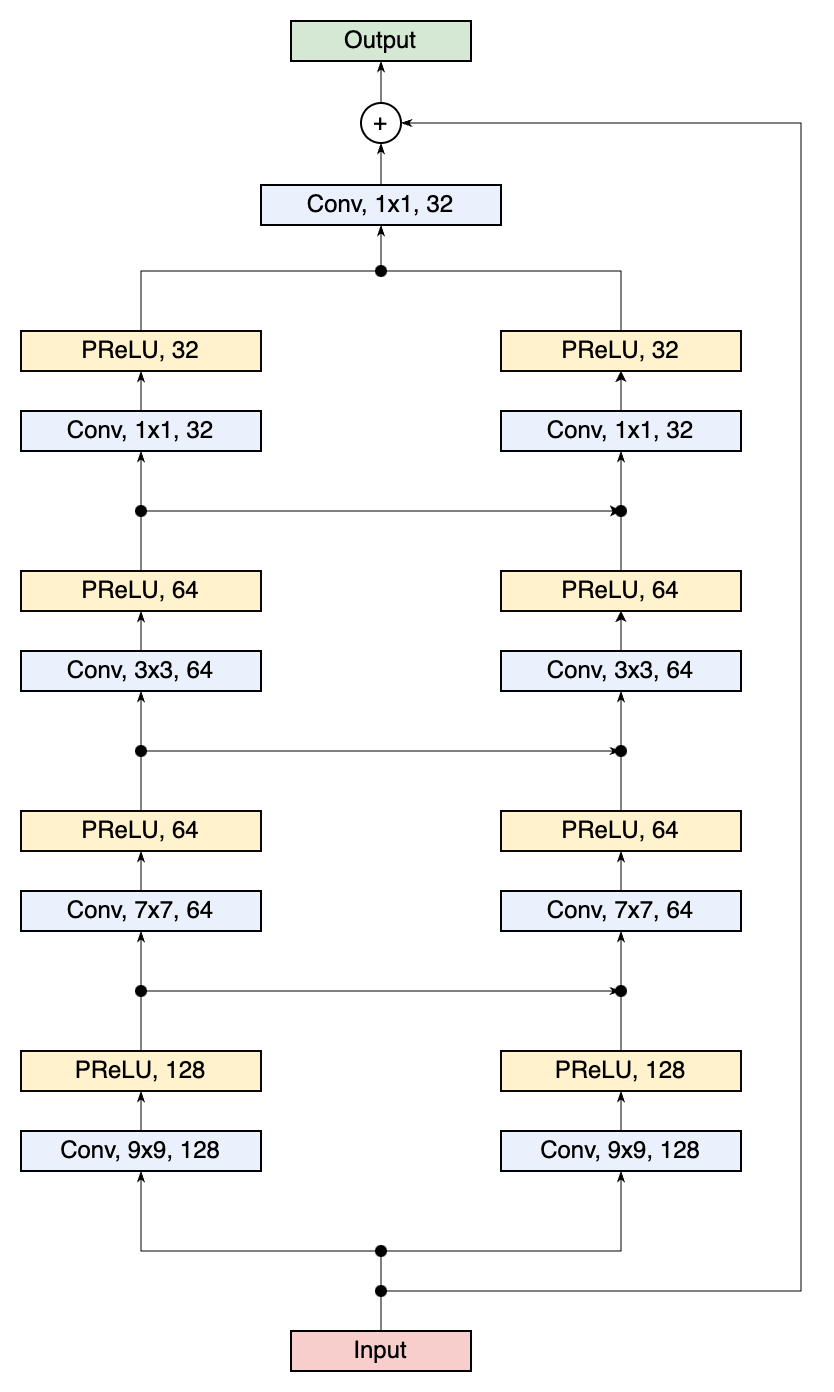
\includegraphics[width=10cm]{./images/model-architecture.png}
    \caption{Архитектура предлагаемой нейронной сети}
    \label{model-architecture}
\end{figure}

\subsection{Функция потерь}\label{subsection:loss-function}

При работе с изображениями чаще всего используется функция потерь MSE (Mean Squared Error)~\cite{ar-cnn-overview,qe-cnn-overview}. Если $\{I_n\}_{n=1}^N$ --- набор исходных изображений, $\{\tilde{I}_n\}_{n=1}^N$ --- множество из тех же изображений но с частично обнуленными ДКП коэффициентами, $\Theta=\{W_i, B_i, a_i\}$ --- обучаемые параметры модели $M$, то
\[
    MSE(\Theta) = \dfrac{1}{N} \sum_{n=1}^N \left( M(\tilde{I}_n, \Theta) - I_n \right)^2.
\]
При обучении требуется минимизировать данную функцию потерь, например, с помощью модификаций алгоритма градиентного спуска.

\chapterconclusion

В данной главе был рассмотрен алгоритм транскодирования JPEG-изображений на основе нейронной сети, а именно причины выбора такого метода внутреннего предсказания, общая идея алгоритма и все преобразования, которые происходят с изображением в процессе его работы. Отдельное внимание было уделено требованиям к этапу обнуления коэффициентов и архитектуре нейронной сети.

\chapter{Реализация и тестирование}\label{chapter:implementation-and-testing}

В данной главе описан процесс разработки транскодера, нейронной сети и ее обучения, подготовка набора данных, параметры обучения, а также алгоритм тестирования транскодера, результаты его работы и их анализ.

\section{Разработка транскодера JPEG}\label{section:transcoding-implementation}

Данный раздел содержит описание реализации всех этапов транскодирования изображений, кроме внутреннего предсказания.

\subsection{Публичное C++ API транскодера}\label{subsection:decoder-cpp-api}

Для обработки JPEG-изображений на C++ был разработан класс \texttt{Decoder}, реализующий следующие режимы работы:
\begin{enumerate}
    \item \texttt{Decoder::Mode::DEFAULT} --- стандартное декодирование JPEG в PPM (установлен по умолчанию);
    \item \texttt{Decoder::Mode::ZERO\_OUT\_AND\_DECODE} --- декодирование JPEG в PPM с частичным обнулением ДКП коэффициентов;
    \item \texttt{Decoder::Mode::ENCODE\_RESIDUALS} --- транскодирование JPEG;
    \item \texttt{Decoder::Mode::DECODE\_RESIDUALS} --- трансдекодирование JPEG.
\end{enumerate}

Публичное API класса \texttt{Decoder} содержит следующие методы:
\begin{enumerate}
    \item \texttt{Decoder \& toggle\_mode(Mode)} --- переключение режима работы;
    \item \texttt{Decoder \& set\_dct\_filter(std::size\_t)} --- настройка числа обнуляемых ДКП-коэффициентов для каждого блока;
    \item \texttt{Decoder \& set\_enhanced\_file(const std::string \&)} --- найстройка пути к PPM файлу, содержащему обработанное нейронной сетью в процессе внутреннего предсказания изображение;
    \item \texttt{void decode(const BytesList \&)} --- декодирование потока байтов из файла JPEG (\texttt{BytesList} является синонимом для \texttt{set::vector<unsigned char>});
    \item \texttt{bool is\_color\_image() const} --- получение информации о том, является ли декодированное изображения цветным;
    \item \texttt{std::size\_t get\_width() const} --- получение ширины изображения;
    \item \texttt{std::size\_t get\_height() const} --- получение высоты изображения;
    \item \texttt{const BytesList \& get\_image() const} --- получение байтов декодированного изображения;
    \item \texttt{const Output \& get\_transcoded() const} --- получение результата транскодирования/трансдекодирования (\texttt{Output} --- класс, инкапсулирующий в себе поток байтов).
\end{enumerate}

Пример создания и настройки декодера представлен на листинге~\ref{listing:decoder-configuration-example}.\par

\begin{lstlisting}[float=!h,caption={Пример создания и настройки декодера},label={listing:decoder-configuration-example}]
Decoder decoder;
decoder
    .toggle_mode(Decoder::Mode::ENCODE_RESIDUALS)
    .set_dct_filter(16)
    .set_enhanced_file("enhanced.ppm");
\end{lstlisting}

\subsection{Интерфейс командной строки}\label{subsection:decoder-cli}

Для удобства работы с декодером был разработан интерфейс командной строки с использованием сторонней библиотеки args~\cite{args-lib}. Он поддерживает такие опции как \texttt{--zero-out-and-decode} (листинг~\ref{listing:zero-out-and-decode-flag}), \texttt{--encode-residuals} (листинг~\ref{listing:encode-residuals-flag}), \texttt{--decode-residuals} (листинг~\ref{listing:decode-residuals-flag}), соответсвующие одноименным режимам работы. Если ни одна из перечисленных опций не передана --- запускается обычное декодирование JPEG в PPM (листинг~\ref{listing:default-cli}).

\begin{lstlisting}[float=!h,caption={Пример вызова декодера для декодирования JPEG с частичным обнулением коэффициентов ДКП},label={listing:zero-out-and-decode-flag}]
$ ./Decoder --zero-out-and-decode --input "input.jpeg" --output "output.ppm" --power 16
\end{lstlisting}

\begin{lstlisting}[float=!h,caption={Пример вызова декодера для транскодирования},label={listing:encode-residuals-flag}]
$ ./Decoder --encode-residuals --input "original.jpeg" --output "compressed.jpeg" --enhanced "enhanced.ppm" --power 16
\end{lstlisting}

\begin{lstlisting}[float=!h,caption={Пример вызова декодера для трансдекодирования},label={listing:decode-residuals-flag}]
$ ./Decoder --decode-residuals --input "compressed.jpeg" --output "original.jpeg" --enhanced "enhanced.ppm" --power 16
\end{lstlisting}

\begin{lstlisting}[float=!h,caption={Пример вызова декодера для декодирования JPEG},label={listing:default-cli}]
$ ./Decoder --input "input.jpeg" --output "output.ppm"
\end{lstlisting}

\subsection{Детали реализации этапа обнуления коэффициентов}\label{subsection:decoder-implementation-details}

Для обнуления части коэффициентов был реализован класс \texttt{utils::DCTCoefficientsFilter}. Объекты данного класса инициализируются следующими параметрами:
\begin{enumerate}
    \item \texttt{power} --- число обнуляемых коэффициентов;
    \item \texttt{masks\_count} --- число различных наборов коэффициентов (значение по умолчанию: 9);
    \item \texttt{seed} --- зерно для инициализации генератора псевдослучайных чисел (значение по умолчанию: 42).
\end{enumerate}

В конструкторе объекта данного класса создается \texttt{masks\_count} псевдослучайных битовых масок длины 64 (\texttt{std::bitset<64>}), содержащих нули ровно на \texttt{power} позициях. Для получения маски используется метод \texttt{std::bitset<64> utils::DCTCoefficientsFilter::get\_mask()}, который автоматически переходит к следующей по счету маске при каждом обращении. После получения всех масок счетчик сбрасывается. Пример использования данного класса показан на листинге~\ref{listing:dct-coefficients-filter}.

\begin{lstlisting}[float=!h,caption={Пример использования класса для обнуления коэффициентов},label={listing:dct-coefficients-filter}]
utils::DCTCoefficientsFilter filter(16);
const auto mask = filter.get_mask();
\end{lstlisting}

\subsection{Детали реализации кодирования коэффициентов}\label{subsection:residuals-processing-implementation-details}

Для транскодирования и трансдекодирования декодеру требуется предоставить PPM-изображение, содержащее изображение после этапа внутреннего предсказания, то есть обработанное нейронной сетью. Транскодирование каждого блока изображения осуществляется независимо. При обработке блока, начальная точка которого имеет координаты $(x,\ y)$:
\begin{enumerate}
    \item Из PPM-изображения вырезается соответствующий фрагмент (с теми же координатами), переводится в YCbCr и из него выбирается яркостный компонент (листинг~\ref{listing:cut-enhanced-block});
          \begin{lstlisting}[float=!h,caption={Получение фрагмента изображения после внутреннего предсказания},label={listing:cut-enhanced-block}]
std::array<float, 64> image_fragment;
for (std::size_t pixel_x = 0, k = 0; pixel_x < 8; ++pixel_x) {
    for (std::size_t pixel_y = 0; pixel_y < 8; ++pixel_y, ++k) {
        image_fragment[k] = m_enhanced_file->get_yuv(x + pixel_x, y + pixel_y).m_luminance;
    }
}
    \end{lstlisting}
    \item Далее к вырезанному блоку применяется ДКП (листинг~\ref{listing:dct-enhanced-block});
          \begin{lstlisting}[caption={Применение прямого ДКП},label={listing:dct-enhanced-block}]
utils::DiscreteCosineTransform::forward(image_fragment);
    \end{lstlisting}
    \item Затем блок квантуется с использованием таблицы для яркостного компонента исходного JPEG-изображения. Реализация данного метода приведена на листинге~\ref{listing:enhanced-block-quantization}.
          \begin{lstlisting}[caption={Квантование блока},label={listing:enhanced-block-quantization}]
m_quantization_tables
        .at(component.m_quantization_table_id)
        .forward(image_fragment);
    \end{lstlisting}
\end{enumerate}

Далее после декодирования блока исходного JPEG-изображения, в нем происходит замена обнуляемых коэффициентов на основании маски \texttt{mask}, полученной из объекта \texttt{utils::DCTCoefficientsFilter}, на разницу между исходными коэффициентами и предсказанными (в режиме \texttt{Decoder::Mode::ENCODE\_RESIDUALS}) или на сумму закодированной ошибки предсказания и предсказанного коэффициента (для \texttt{Decoder::Mode::DECODE\_RESIDUALS}). Фрагмент кода, реализующий данные операции представлен на листинге~\ref{listing:replacement-dct-coefficients-with-residuals}.

\begin{lstlisting}[float=!h,caption={Замена коэффициентов ДКП на ошибки предсказания и наоборот},label={listing:replacement-dct-coefficients-with-residuals}]
for (std::size_t i = 1; i < 64; ++i) {
    if (mask[i]) {
        continue;
    }
    if (IsEncodeResidualsMode()) {
        // Replace DCT coefficient with residual:
        block[i] -= enhanced_block[i];
    }
    else {
        // Recovery of the DCT coefficient based on the residual and the predicted value:
        block[i] += enhanced_block[i];
    }
}
\end{lstlisting}

\section{Разработка нейронной сети}\label{section:model-implementation}

Для разработки и обучения нейронной сети была использована библиотека машинного обучения для Python --- PyTorch~\cite{pytorch}. В данном разделе описаны детали реализации и обучения QE-CNN-P.

\subsection{Реализация QE-CNN-P}\label{subsection:model-implementation}

Реализация QE-CNN-P представлена классом \texttt{quality\_enhancement.models.QECNN}, базовым классом которого является \texttt{torch.nn.Module}. Слои нейронной сети реализованы с помощью \texttt{torch.nn.Sequential} API и классов \texttt{torch.nn.Conv2d} (двумерная свертка) и \texttt{torch.nn.PReLU} (функция $PReLU$, описанная в разделе~\ref{subsection:qe-cnn}).\par

Для того, чтобы каждый слой модели сохранял размерность входного изображения, использовалась следующая формула рассчета отступа $P$ для свертки
\[
    P = \left\lfloor\dfrac{n - 1}{2}\right\rfloor,
\]
где $n$ --- размер ядра свертки.

\subsection{Подготовка набора данных}\label{subsection:dataset-preparing}

Для обучения нейронной сети было взято $50000$ случайных изображений из набора данных ImageNET~\cite{image-net}, из которых 5000 было выделено для тестирования модели, 10000 --- для валидации и оставшиеся 35000 --- для обучения. Изображения были обрезаны до размера $320\times320$, затем в каждом блоке $8\times8$ пикселей были удалены (заменены нулями) по 16 псевдослучайных AC-коэффициентов, как это было описано в разделе~\ref{section:zeroing-the-coefficients}.\par

Для упрощения обработки большого числа изображений был реализован скрипт \texttt{image\_processing.py} на Python. Так в примере, указанном на листинге~\ref{listing:image-processing-example}, сначала происходит разметка изображений по их принадлежности к определенной части набора данных (в зависимости от назначения), затем файлы обрезаются до необходимого размера и каждый из них декодируется в двух режимах --- стандартном и с обнулением коэффициентов. Полученные изображения были использованы для обучения модели.

\begin{lstlisting}[float=!h,caption={Подготовка набора данных для обучения модели},label={listing:image-processing-example}]
$ python3 py/process_images.py --split -i "images/01-original-images" --validation_size 0.2 --test_size 0.1
$ python3 py/process_images.py --crop -i "images/01-original-images" -o "images/02-croped" --height 320 --width 320
$ python3 py/process_images.py --decode -i "images/02-croped" -o "images/03-decoded"
$ python3 py/process_images.py --zero_out_and_decode -i "images/02-croped" -o "images/04-decompressed" --power 16
\end{lstlisting}

\subsection{Параметры обучения}\label{subsection:learning-parameters}

Обучение производилось на персональном компьютере MacBook Pro 2021 г. (чип Apple M1 Pro) на основании функции ошибки MSE (\texttt{torch.nn.MSELoss}) с использованием оптимизатора Adam (\texttt{torch.optim.Adam}) с параметром $learning\_rate=1\mathrm{e}{-4}$ на протяжении 100 эпох. После каждой эпохи рассчитывалась метрика MSE на валидационном наборе данных. Наименьшее значение функции ошибки было достигнуто по завершении последней эпохи и составило $1,405\mathrm{e}{-3}$.\par

\subsection{Интерфейс командной строки}\label{subsection:model-cli}

Для удобства работы с моделью был реализован интерфейс командной строки. В нем поддерживаются две опции:
\begin{enumerate}
    \item \verb|--train| --- запуск обучения нейронной сети;
    \item \verb|--enhance| --- обработка изображений для их транскодирования.
\end{enumerate}

Для запуска обучения модели требуется настройка следующих параметров (пример показан на листинге~\ref{listing:train-model-example}):
\begin{enumerate}
    \item \verb|--limit| --- ограничение на размер набора данных;
    \item \verb|--learning_rate| --- скорость обучения;
    \item \verb|--checkpoints_folder| --- путь к папке, содержащей чекпоинты, то есть файлы, содержащие словари состояний параметров модели и оптимизатора.
\end{enumerate}

\begin{lstlisting}[float=!h,caption={Пример запуска обучения модели},label={listing:train-model-example}]
$ python3 py/main.py --train --limit 3600 --learning_rate=0.0001 --checkpoints_folder "py/checkpoints"
\end{lstlisting}

Для запуска внутреннего предсказания модели необходимо настроить (листинг~\ref{listing:enhance-example}):
\begin{enumerate}
    \item \verb|--input_wildcard|/\verb|-I| --- шаблон файлов, которые требуется обработать;
    \item \verb|--output_folder|/\verb|-O| -- папка, в которую необходимо сохранить обработанные изображения;
    \item \verb|--checkpoints_folder| --- путь к папке, содержащей чекпоинты.
\end{enumerate}

\begin{lstlisting}[float=!h,caption={Пример запуска внутреннего предсказания},label={listing:enhance-example}]
$ python3 py/main.py --enhance -I "images/decompressed/tst*.ppm" -O "images/enhanced" --checkpoints_folder "py/checkpoints"
\end{lstlisting}

\section{Тестирование}\label{section:testing}

\subsection{Оценка качества работы нейронной сети}\label{subsection:model-testing}

На рисунке~\ref{image:image-transformation-example} проиллюстрировано то, насколько хорошо обученная модель справляется с искажениями, которые были внесены в результате обнуления коэффициентов. На примере видно, что большая часть видимых искажений устранена. Так, например, на левом изображении практически на всех участках четко видно деление на блоки, а после нейросетевой обработки подобных артефактов уже не остается. Таким образом, визуально заметно, что нейросети удается приближенно восстанавливать обнуленные ДКП коэффициенты.

\begin{figure}[!h]
    \centering
    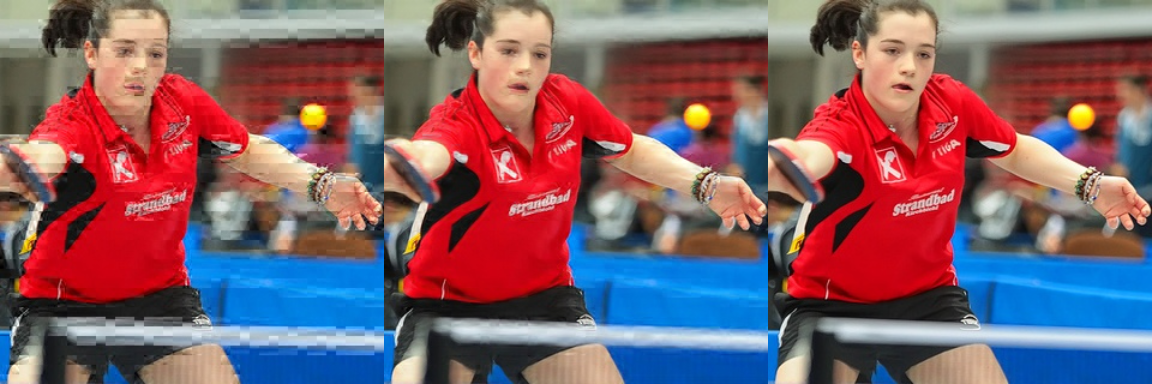
\includegraphics[width=\textwidth]{./images/image-transformation-example.png}
    \caption{Пример работы QE-CNN: слева --- изображение после обнуления части ДКП коэффициентов; посередине --- изображение на выходе нейронной сети; справа — исходное изображение}
    \label{image:image-transformation-example}
\end{figure}

Графики на рисунке~\ref{image:coefficients_distribution} показывают сравнение распределений ошибок предсказания коэффициентов ДКП (residuals) на позициях обнуленных коэффициентов и самих этих коэффициентов для позиций 6, 7, 12, 13, 21 и 22 (означающих индексы AC-коэффициентов при сканировании в зигзагообразном порядке). Видно, что ошибки предсказания сконцентрированы ближе к нулю, чем сами коэффициенты. Следовательно, число ненулевых кодируемых энтропийным кодером значений сокращается, а их абсолютные значения уменьшаются. На основании этого можно сделать вывод о том, что их энтропия снижается и итоговый объем битового потока должен быть меньше.

\begin{figure}[!h]
    \centering
    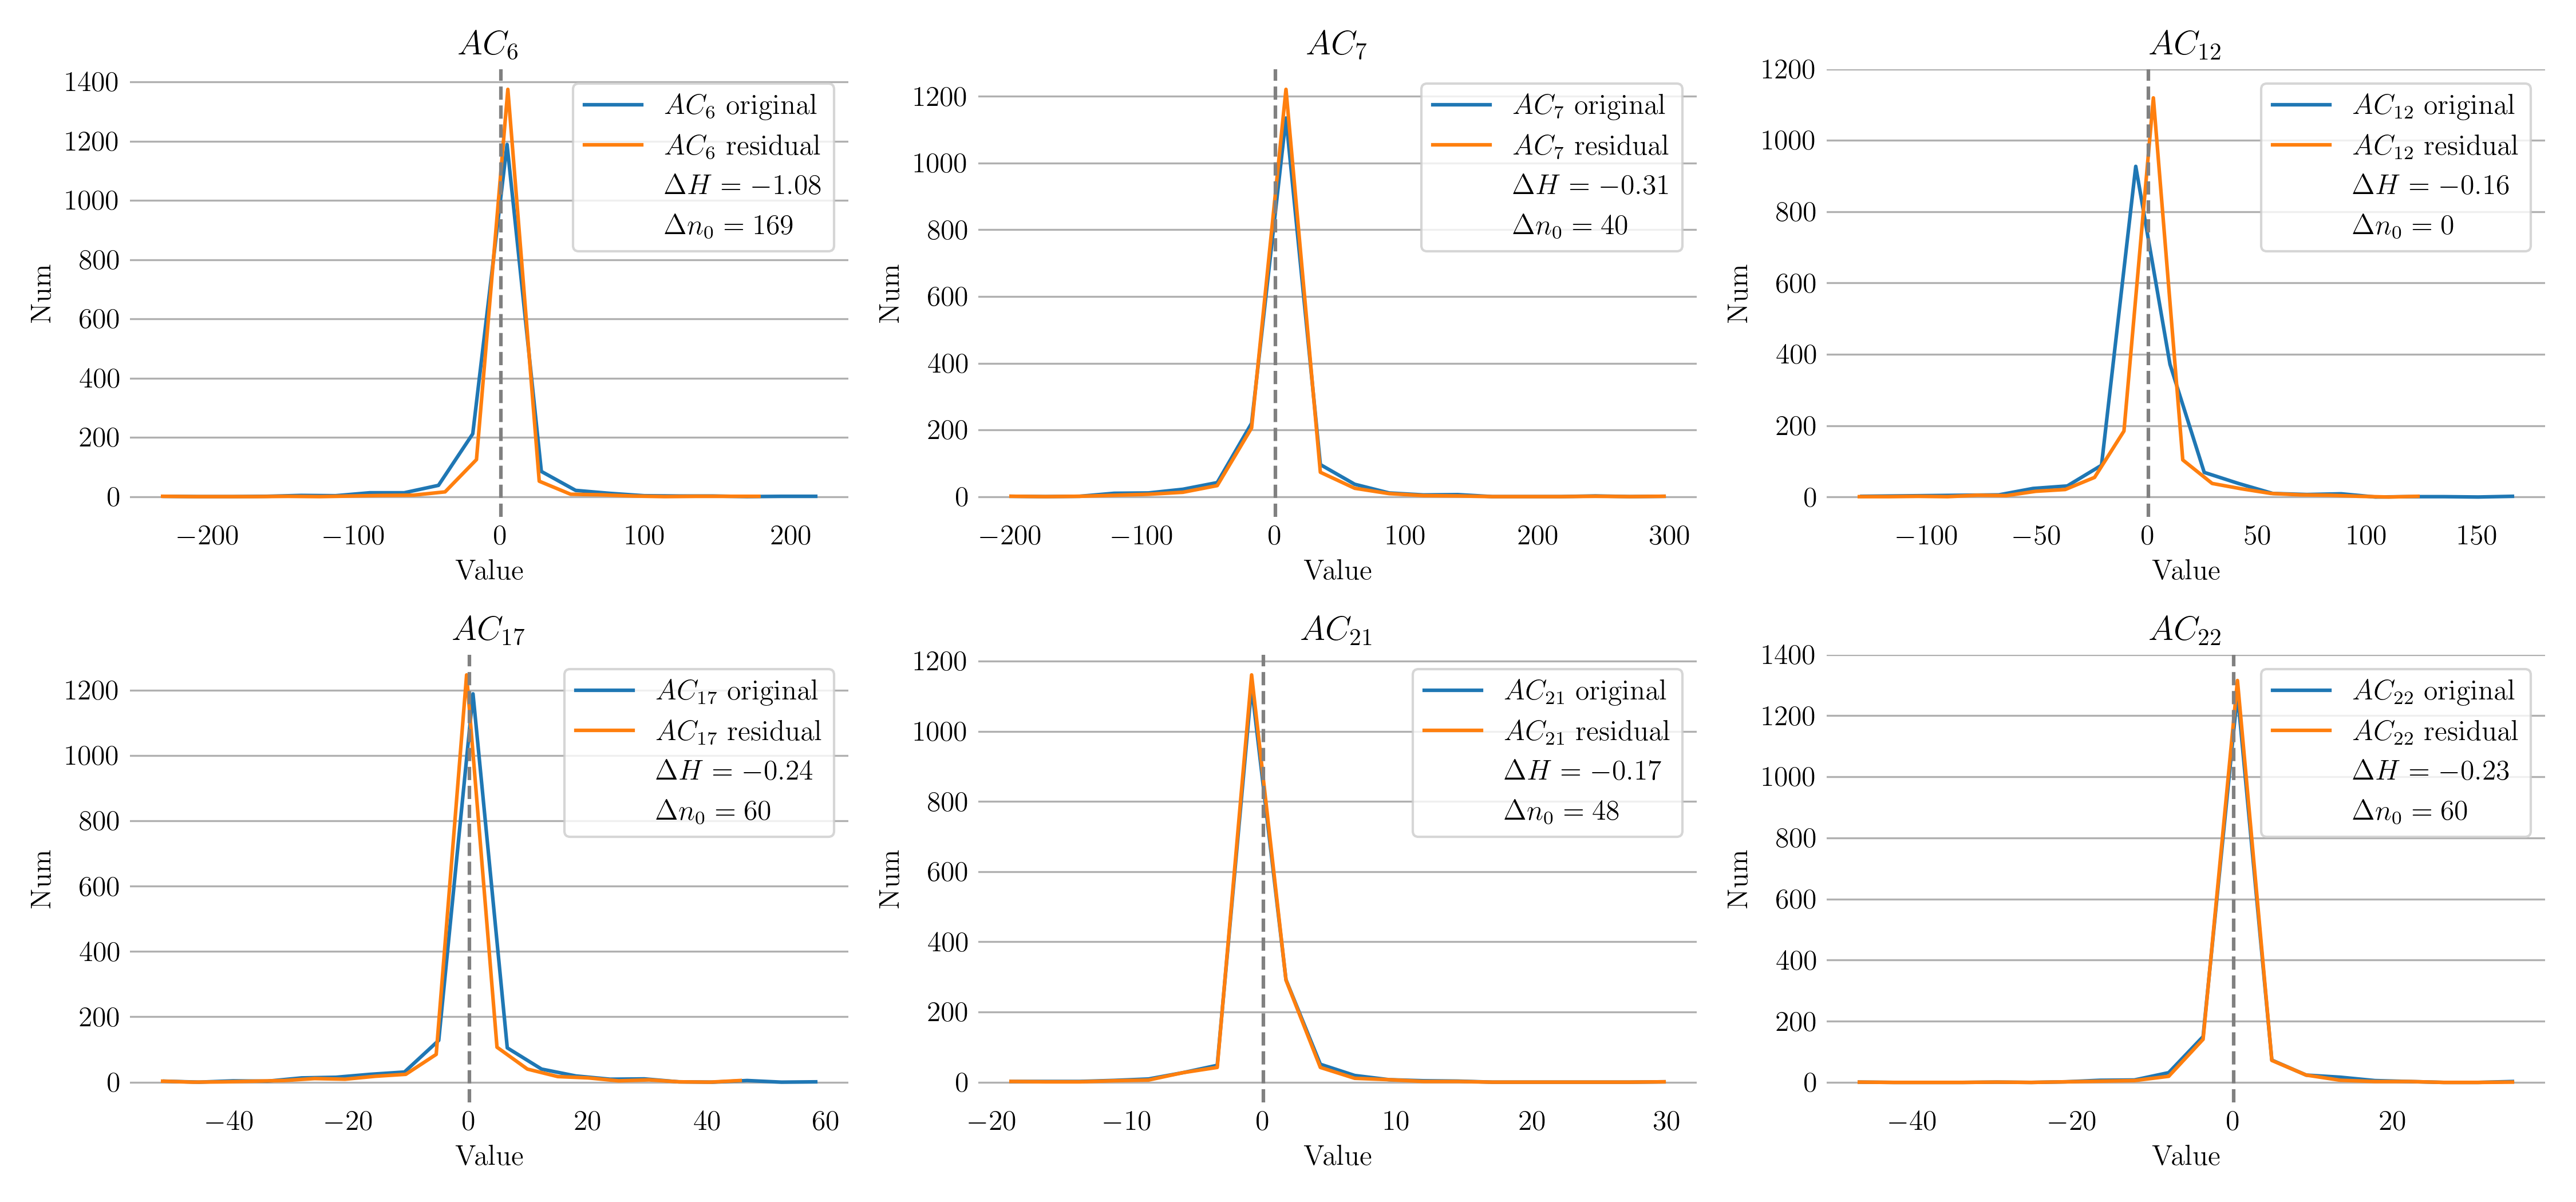
\includegraphics[width=\textwidth]{./images/coefficients_distribution.png}
    \caption{Распределение обнуляемых AC-коэффициентов и ошибок их предсказаний на изображении из тестового набора данных, показанном на рисунке~\ref{image:image-transformation-example} при обнулении 16 коэффициентов, $\Delta H$ --- изменение энтропии, $\Delta n_0$ --- изменение числа нулевых значений коэффициентов}
    \label{image:coefficients_distribution}
\end{figure}

\subsection{Подготовка набора транскодированных и трансдекодированных изображений}\label{subsection:testing}

Для выполнения функционального тестирования реализованного транскодера, оценки степени сжатия изображений и анализа возможности интеграции предлагаемого модуля внутреннего предсказания с утилитами Jpegtran и LLJPEG был доработан скрипт \texttt{image\_processing.py}. В него были добавлены функции транскодирования (листинг~\ref{listing:transcoding-example}) и трансдекодирования (листинг~\ref{listing:transdecoding-example}) набора изображений, применения Jpegtran к JPEG-изображениям с целью замены кода Хаффмана на арифметический кодер (листинг~\ref{listing:arithmetic-example}), функции расчета статистики изображений: средней, медианной и максимальной степеней сжатия (листинг~\ref{listing:statistics-example}), а также опция для запуска end-to-end тестов транскодера (листинг~\ref{listing:end-to-end-tests}).

\begin{lstlisting}[float=!h,caption={Пример транскодирования набора изображений},label={listing:transcoding-example}]
$ python3 py/process_images.py --encode_residuals -i "images/02-croped" -o "images/06-transcoded" -e "images/05-enhanced" --power 16
\end{lstlisting}

\begin{lstlisting}[float=!h,caption={Пример трансдекодирования набора изображений},label={listing:transdecoding-example}]
$ python3 py/process_images.py --decode_residuals -i "images/06-transcoded" -o "images/07-transdecoded" -e "images/05-enhanced" --power 16
\end{lstlisting}

\begin{lstlisting}[float=!h,caption={Пример транскодирования набора изображений, основанного на замене кода Хаффмана на арифметический кодер},label={listing:arithmetic-example}]
$ python3 py/process_images.py --arithmetic -i "images/02-croped" -o "images/08-jpegtran-output"
$ python3 py/process_images.py --arithmetic -i "images/06-transcoded" -o "images/09-jpegtran-output-for-transcoded"
\end{lstlisting}

\begin{lstlisting}[float=!h,caption={Пример рассчета статистики сжатия изображений},label={listing:statistics-example}]
$ python3 py/process_images.py --statistics -i "images/02-croped" -o "images/06-transcoded"
$ python3 py/process_images.py --statistics -i "images/02-croped" -o "images/08-jpegtran-output"
$ python3 py/process_images.py --statistics -i "images/02-croped" -o "images/09-jpegtran-output-for-transcoded"
\end{lstlisting}

\begin{lstlisting}[float=!h,caption={Пример запуска end-to-end тестов транскодера},label={listing:end-to-end-tests}]
$ python3 py/process_images.py --test_transcoder -i "images/02-croped" -o "images/07-transdecoded"
Test result: succeeded
\end{lstlisting}

\subsection{Детали реализации end-to-end тестирования}\label{section:functional-testing}

Функциональное end-to-end тестирование транскодера основано на сравнении файлов до и после транскодирования с точностью до бита. Для этого используется функция стандартной библиотеки Python --- \texttt{filecmp.cmp}, которая принимает пути к двум файлам и возвращает \texttt{True}, если они совпадают.\par

Тестрование проводилось на том же тестовом наборе данных, на каком оценивалась эффективность работы транскодера, и было завершено без ошибок.

\subsection{Оценка степени сжатия}\label{subsectiong:compressing-testing}
Оценка качества работы транскодера выполнялась на упомянутом выше тестовом наборе данных. Были рассмотрены следующие варианты транскодирования изображений (результаты экспериментов представлены в таблице~\ref{table:compression-cmp}):
\begin{enumerate}
    \item \textit{Предобученная модель} --- метод транскодирования, использующий для внутреннего предсказания модель QE-CNN-P обученную для визуального повышения качества изображений~\cite{ai-video-enhancement} и видео, закодированных кодеком HEVC;
    \item \textit{Предложенный 1} (CNN-based) --- метод транскодирования на внутреннего предсказания с помощью обученной в рамках настоящей работы модели машинного обучения;
    \item \textit{Jpegtran};
    \item \textit{Предложенный 2} (CNN-based + Jpegtran) --- комбинация CNN-based и Jpegtran;
    \item \textit{LLJPEG};
    \item \textit{Предложенные 3} (CNN-based + LLJPEG) --- комбинация CNN-based и LLJPEG.
\end{enumerate}

\begin{table}[!h]
    \caption{Сравнение степени сжатия, \%}\label{table:compression-cmp}
    \centering
    \begin{tabular}{|*{6}{c|}}\hline
        \diagbox{Методы}{Метрики} & Среднее & Медиана & $\sigma$ & По всему набору данных \\\hline
        Предобученная модель      & 2,57    & 2,68    & 0,87     & 2,76                   \\\hline
        Предложенный 1            & 3,33    & 3,38    & 0,54     & 3,38                   \\\hline
        Jpegtran                  & 10,05   & 10,00   & 3,06     & 10,12                  \\\hline
        Предложенный 2            & 13,16   & 13,11   & 2,91     & 13,18                  \\\hline
        LLJPEG                    & 16,14   & 15,49   & 3,37     & 15,59                  \\\hline
        Предложенный 3            & 15,44   & 15,08   & 2,61     & 15,14                  \\\hline
    \end{tabular}
\end{table}

Результаты эксперимента показывают, что обученная в рамках настоящей работы нейронная сеть сжимает тестовый набор изображений на 3,38\% (в отличие от предобученной нейронной сети с такой же архитектурой, но решающей иную задачу). На рисунке~\ref{image:bitrade-distribution} также можно видеть, что большинство изображений сжаты 1-м предложенным методом на 3-4\% и отклонение от этой статистики небольшое (о чем и говорит низкое стандартное оклонение). Лишь на единицах изображений описанный подход к транскодированию оказался неэффективным.

\begin{figure}[!h]
    \centering
    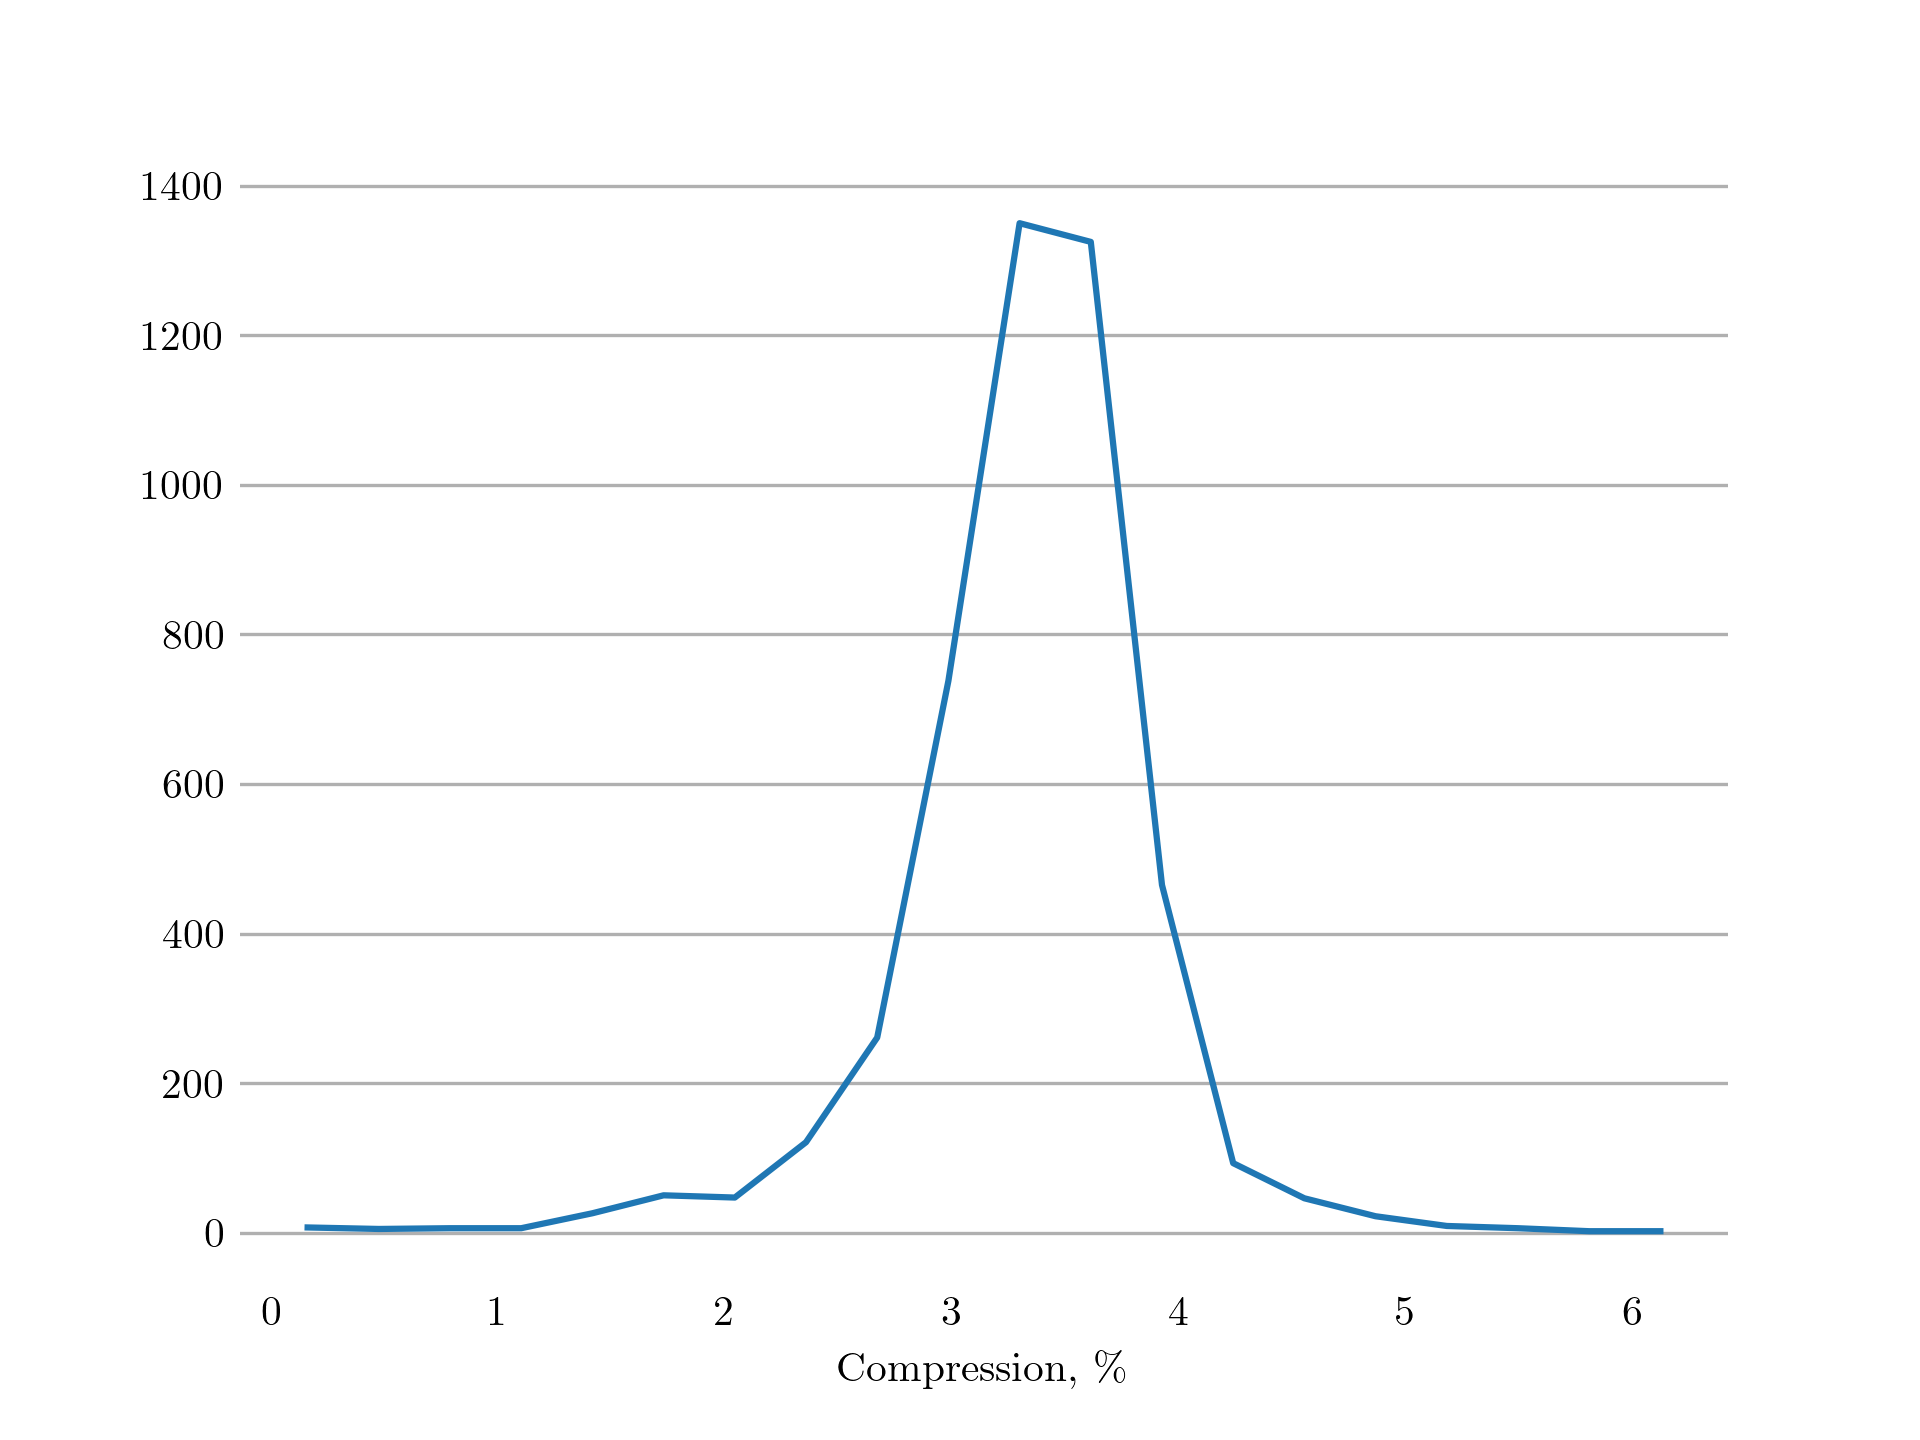
\includegraphics[width=13cm]{./images/bitrade_distribution.png}
    \caption{Кривая, показывающая для какого числа изображений из тестового набора удалось достичь определенной степени сжатия}
    \label{image:bitrade-distribution}
\end{figure}

Таким образом, результаты экспериментов показывают, что предлагаемый в настоящей работе метод предсказания коэффициентов ДКП хорошо комбинируется с Jpegtran, позволяющим заменить код Хаффмана на арифметический код. Степени сжатия, наблюдаемые при использовании каждого из этих подходов, фактически суммируются, если использовать методы совместно.\par

Несмотря на то, что на практике транскодер LLJPEG показывает наилучшие результаты, 2-й предлагаемый метод отстает от него всего на 2,41\% (при рассмотрении сжатия всего тестого набора данных в целом). При этом в данной комбинации реализовано только предсказание AC-коэффициентов и улучшение энтропийного кодера благодаря использованию арифметического кодирования, что необходимо учитывать при сравнении эффективности работы двух данных подходов.

\subsection{Дальнейшие перспективы исследования}\label{chapter:prospects}

Как было упомянуто в предыдущем разделе --- рассмотренный в настоящей работе транскодер реализует только часть из известных на сегодняшний день подходов, причем целью исследования являлось изучение конкретного этапа --- внутреннего предсказания, и возможности использования нейронной сети на данном этапе. Отдельно требуется отметить, что из-за ограничений на вычислительные ресурсы при подготовке работы:
\begin{enumerate}
    \item Не выполнена оптимизация числа обнуляемых коэффциентов --- эксперименты проводились для изображений, в которых удалены 16 AC-коэффициентов;
    \item Не проведены эксперименты для разных параметров качества (quality factor, QF);
    \item Нейронная сеть была обучена на небольшом числе изображений и эпох (анализ научных статей на тему кодирования изображений при помощи нейронных сетей~\cite{jeon2023contextbased, feng2023nvtc, huang2023accurate} показывает, что набор данных обычно содержит не менее 90'000 изображений, а обучение проводится на протяжении 1-2 млн. эпох);
    \item Не оптимизированы архитектуры нейронной сети и функции потерь.
\end{enumerate}

Несмотря на все вышеупомянутые ограничения результаты показывают, что нейронные сети можно использовать для предсказания коэффициентов ДКП и что такой метод позволяет добиваться дополнительного сжатия JPEG. Для увеличения степени сжатия в рамках дальнейшей работы над нейросетевым транскодером планируется:
\begin{enumerate}
    \item Продолжать обучение нейронной сети (в идеале с использованием больших вычислительных ресурсов);
    \item Оценить степень сжатия для различных гиперпараметров алгоритма; например, иного числа удаляемых коэффициентов, большего числа битовых масок;
    \item Рассмотреть возможность нейросетевого внутреннего предсказания DC, а не AC коэффициентов;
    \item Доработать алгоритм JPEG на остальных этапах:
          \begin{enumerate}
              \item Ввести адаптивную величину блока;
              \item Внедрить в транскодер адаптивное арифметическое кодирование.
          \end{enumerate}
\end{enumerate}

\chapterconclusion

В данной главе были рассмотрены детали реализации транскодера, а именно --- C++ API для транскодирования JPEG-изображений, реализация нейронной сети, интерфейсы командной строки для обработки изображений, обучения и запуска модели. Были описаны методики функционального end-to-end тестирования, а также приведены результаты экспериментов по оценке степени сжатия различными алгоритмами транскодирования. Дополнительно была доказана возможность и эффективность интеграции нейросетевого внутреннего предсказания и утилиты Jpegtran.

%% Заключение.
\startconclusionpage

В настоящей работе был проведен анализ тенденций в области сжатия изображений, рассмотрены современные методы кодирования изображений с потерями и без. Было показано, почему этим методы не подходят для дополнительного сжатия JPEG без потерь и рассмотрены существующие подходы к решению данной задачи. При анализе методов были выделены общие положения, определяющие то, на каких этапах возможна реализация транскодирования JPEG без потерь.\par

Был предложен алгоритм транскодирования без потерь, использующий внутреннее предсказание коэффициентов ДКП на основе нейронной сети, для оптимизации облачного хранения изображений, закодированных в формате JPEG. Эксперименты показывают, что такой подход позволяет сократить в среднем 3,33\% (до 6,28\%) памяти на изображениях из подмножества набора данных ImageNET.\par

Несмотря на то, что альтернативные системы транскодирования JPEG-изображений, такие как LLJPEG, позволяют добиться более высокого сжатия, данный подход имеет место быть и нуждается в дальнейшем исследовании, так как в результате его работы получается корректный файл JPEG. Это означает, что данный подход может быть использован одновременно с другими методами транскодирования. К тому же, предлагаемый алгоритм затрагивает исключительно этап внутреннего предсказания, следовательно, он открыт к дальнейшему улучшению, например, за счет отказа от фиксированного размера блока и использования арифметического кодера. Перспективы такого подхода подтверждаются экспериментами по интеграции предлагаемого метода и утилиты Jpegtran.\par

Результатом работы стал программый код транскодера JPEG-изображений без потерь, обученная нейронная сеть, решающая задачу внутреннего предсказания коэффициентов ДКП, а также ряд скриптов, упрощающих работу с наборами изображений и нейронной сетью.\par

\printmainbibliography

\end{document}
